\documentclass{beamer}

\mode<presentation> {


\usetheme{default}
% \setbeamertemplate{footline} % To remove the footer line in all slides uncomment this line
\setbeamertemplate{footline}[page number] % To replace the footer line in all slides with a simple slide count uncomment this line
\setbeamertemplate{navigation symbols}{} % To remove the navigation symbols from the bottom of all slides uncomment this line
}

\usepackage{graphicx} % Allows including images
\usepackage{booktabs} % Allows the use of \toprule, \midrule and \bottomrule in tables
\usepackage{verbatim}
\usepackage{multicol}

\title[VE215 RC3]{VE215 RC3}
\author{Erdao Liang, Chongye Yang}
\institute[UM-SJTU JI] 
{UM-SJTU JI}
\date{
% \today
June 13, 2023
}

\begin{document}

\AtBeginSection[ ]
{
\begin{frame}{Overview}
    \tableofcontents[sectionstyle=show/shaded,subsectionstyle=show/shaded/hide]
    % \tableofcontents[sectionstyle=show/shaded,subsectionstyle=show/shaded]
 \end{frame}
}

%%%%%%%%%%%%%%%%%%%%%%%%%%%%%%%%%%%%%%%%%%%%%%%%%%%
% TITLE PAGE
\begin{frame}
\titlepage % Print the title page as the first slide
\end{frame}

%%%%%%%%%%%%%%%%%%%%%%%%%%%%%%%%%%%%%%%%%%%%%%%%%%%
% OVERVIEW
% \begin{frame}
% \frametitle{Overview}
% \tableofcontents
% \end{frame}


    %%%%%%%%%%%%%%%%%%%%%%%%%%%%%%%%%%%%%%%%%%%%%%%%%%%
% % BASIC LAWS
% \section{Basic Laws}
    
%     %%%%%%%%%%%%%%%%%%%%%%%%%%%%%
%     \begin{frame}{Nodes, Meshes and Loops}
%     \textbf{Branch:} a single element, such as a voltage source or a resistor
    
%     \textbf{Node:} the point of connection between two or more branches
    
%     \textbf{Loop:} any closed path in a circuit
%     \begin{itemize}
%     \item \textbf{Mesh:} a loop that does not enclose any other 
%     loops, i.e., smallest loop
%     \item \textbf{Independent loop:} a loop that contains at least one branch which is not a part of any other independent loop
%     \end{itemize}
    
    
%     Fundamental theorem of network topology:
%     $$b\text{ (branches)}=l\text{(mesh)}+n\text{ (nodes)}-1$$
%     \end{frame}
    

    
%     %%%%%%%%%%%%%%%%%%%%%%%%%%%%%
%     \begin{frame}{Conductance}
%     \begin{equation*}
%     G=\dfrac{1}{R}=\dfrac{i}{v},\ 
%     1S=1\mho=1A/V
%     \end{equation*}
%     where \textbf{G} is the conductance, \textbf{S} (siemens) is the SI unit of conductance and $\mho$ is the reciprocal ohm.
%     \par
%     some useful formula:
%     $$i=Gv,p=vi=i^{2}R=\dfrac{v^2}{R}=v^{2}G=\dfrac{i^{2}}{G}$$
%     \end{frame}
    
%     %%%%%%%%%%%%%%%%%%%%%%%%%%%%%
%     \begin{frame}{Kirchhoff's Law}
%     \begin{table}[]
%         \centering
%         \begin{tabular}{ccc}
%             \toprule
%             Kirchhoff's Law & Expression & Based on \\
%             \midrule
%             KCL & $\sum i_k = 0$ for a node & Conservation of charge\\
%             KVL & $\sum v_k = 0$ for a mesh & Conservation of energy\\
%             \bottomrule
%         \end{tabular}
%     \end{table}
    
    
%     \begin{multicols}{2}
%         \sectiont{}
%         \begin{figure}
%         \centering
%         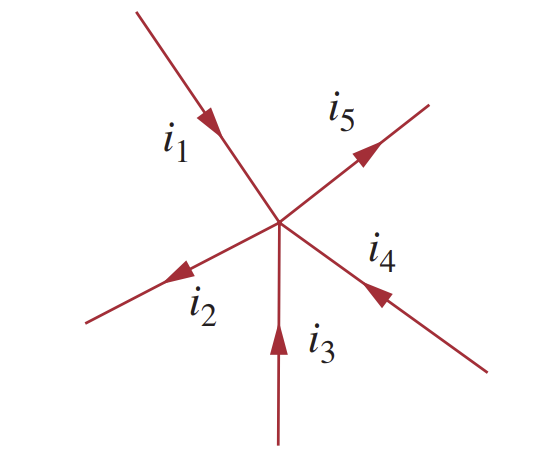
\includegraphics[width=0.33\textwidth]{img_1_to_2/24.png}
%         \caption{KCL}
%         \end{figure}
%         \sectiont{}
%         \begin{figure}
%             \centering
%             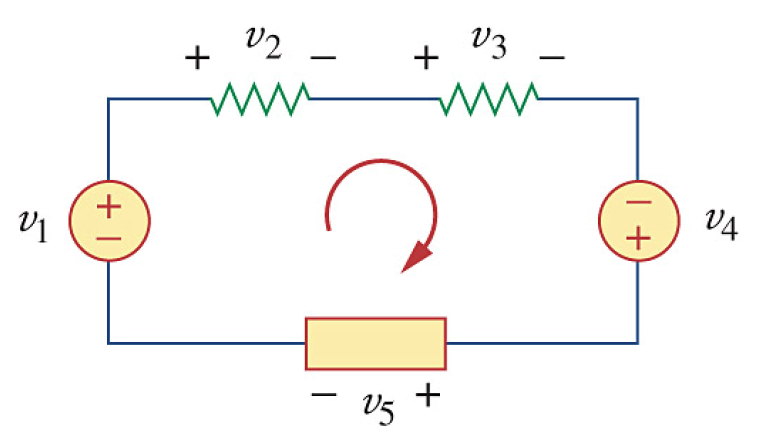
\includegraphics[width=0.48\textwidth]{img_1_to_2/25.png}
%             \caption{KVL}
%         \end{figure}
        
        
%     \end{multicols}
%     \end{frame}
    
%     %%%%%%%%%%%%%%%%%%%%%%%%%%%%%
%     \begin{frame}{KCL}
%     \textbf{KCL:} the algebraic sum of currents entering \textbf{a node (or a closed boundary)} is zero.
    
%     Steps of applying KCL:
%     \begin{enumerate}
%         \item Find out all branches connected to the node of interest.
%         \item Specify \textbf{reference} direction for current on each branch.
%         \item Find all $i_k (k=1,2,\cdots,n)$ (Ohm's law $i=\frac{v_a-v_b}{R}$ for linear resistors).
%         \item List the KCL equation $\sum_{k} i_k = 0$.
%     \end{enumerate}
    
    
    
%     \end{frame}
    
%     %%%%%%%%%%%%%%%%%%%%%%%%%%%%%
%     \begin{frame}{KVL}
%     \textbf{KVL:} the algebraic sum of all voltages around \textbf{a closed path (or loop)} is zero.
    
%     Steps of applying KVL:
%     \begin{enumerate}
%         \item Select reference KVL direction (clockwise by convention).
%         \item Confirm/specify the +/- terminal of each branch.
%         \item Find $v_k (k=1,2,\cdots,n)$ for each branch.
%         \item List the KVL equation $\sum_kv_k=0$. Mind that by passive sign convention, the sign in front of a certain term $v_k$ is 
%         \begin{itemize}
%             \item ``+" if the reference KVL direction enters through the positive terminal of the branch.
%             \item ``-" if the reference KVL direction enters through the negative terminal of the branch.
%         \end{itemize}
%     \end{enumerate}
    
%     \end{frame}
    
    
%     %%%%%%%%%%%%%%%%%%%%%%%%%%%%%
%     \begin{frame}{Wye-Delta Transformation}
    
%     \begin{itemize}
%         \item Motivation: simplify the circuits for easier calculation.
    
%         \item Two forms of special circuit connections:
%         \begin{multicols}
%             \sectiont{}
%                 \begin{figure}[H]
%                 \centering
%                 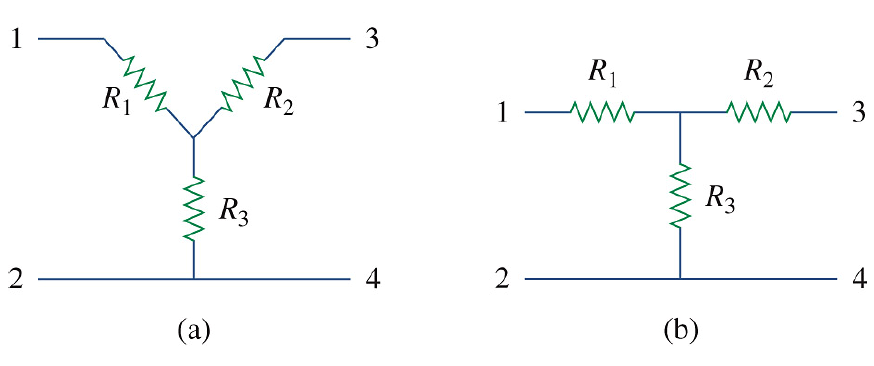
\includegraphics[width=0.45\textwidth]{img_1_to_2/Y.png}
%                 \caption{Wye (Y or T)}
%                 \end{figure}
%             \sectiont{}
%                 \begin{figure}[H]
%                 \centering
%                 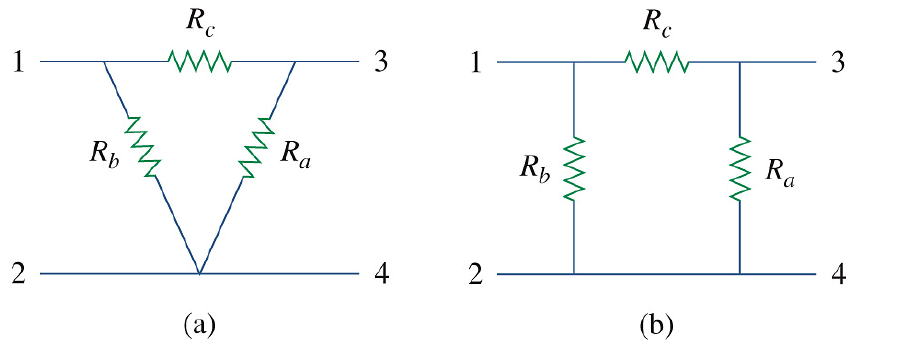
\includegraphics[width=0.5\textwidth]{img_1_to_2/DELTA.png}
%                 \caption{Delta ($\Delta$ or $\pi$)}
%                 \end{figure}
            
%         \end{multicols}
%         \item Goal: transform one type of connection into another.
%     \end{itemize}
    
%     \end{frame}
    
%     %%%%%%%%%%%%%%%%%%%%%%%%%%%%%
%     \begin{frame}{Wye-Delta Transformation}
%     \begin{figure}[H]
%     \centering
%     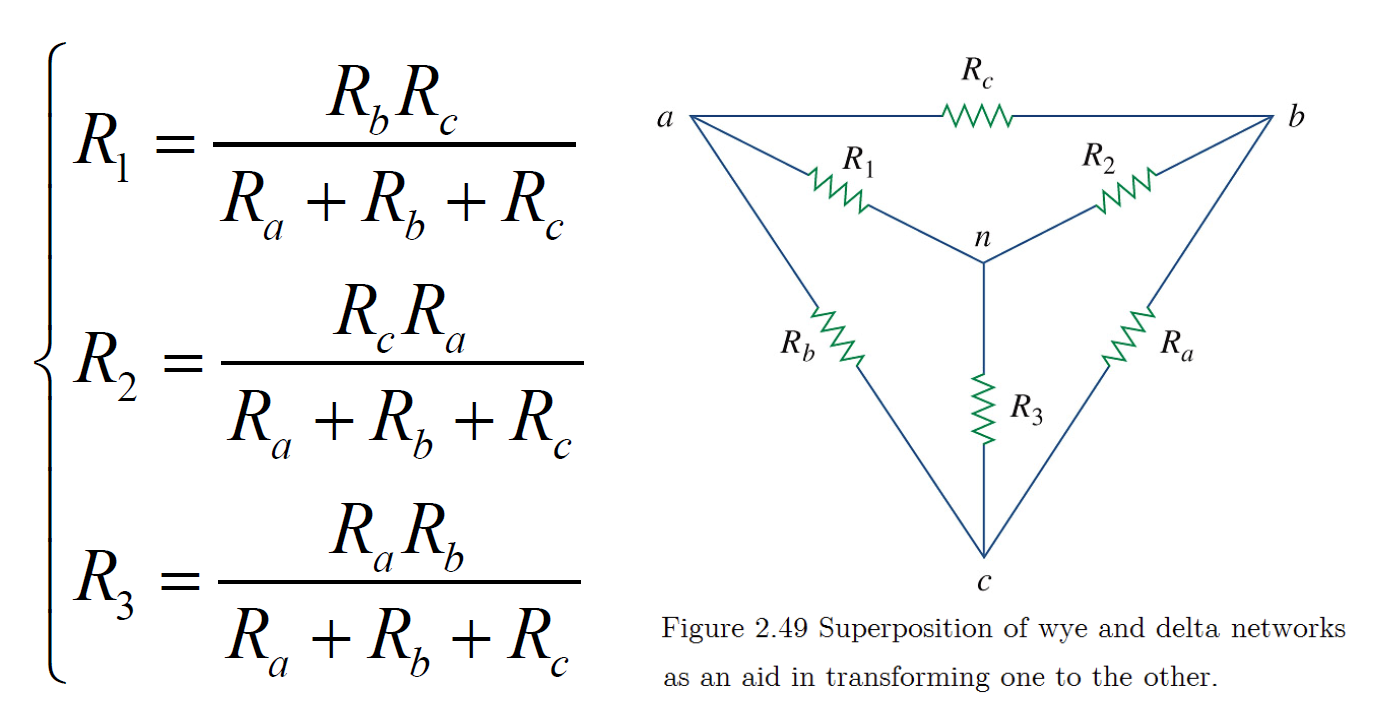
\includegraphics[width=0.7\textwidth]{img_1_to_2/34.png}
%     \caption{\Delta-Y}
%     \end{figure}
    
%     Intuition: parallel $\rightarrow$ series, resistance for each element decreases.
    
%     \end{frame}
    
%     %%%%%%%%%%%%%%%%%%%%%%%%%%%%%
%     \begin{frame}
%     \frametitle{Wye-Delta Transformation}
%     \begin{figure}[H]
%     \centering
%     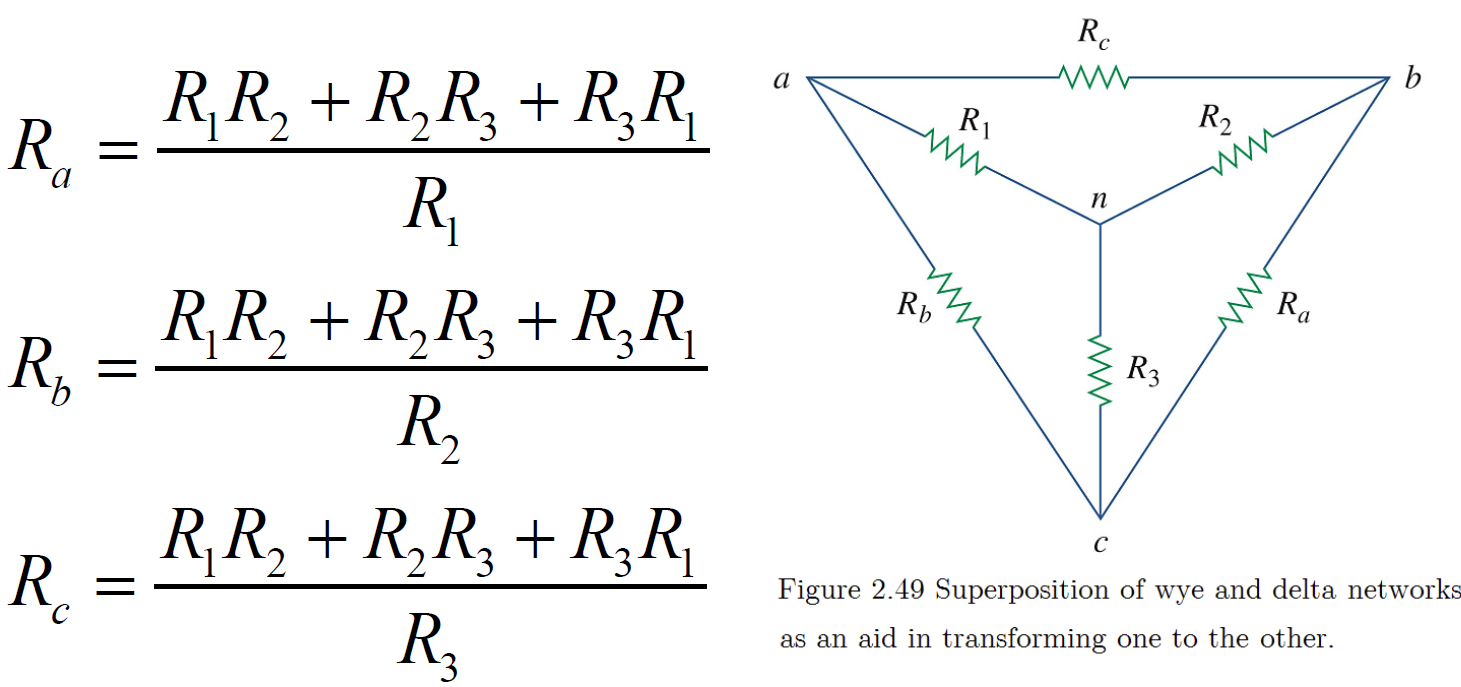
\includegraphics[width=0.7\textwidth]{img_1_to_2/35.png}
%     \caption{Y-\Delta}
%     \end{figure}
    
%     Intuition: series $\rightarrow$ parallel, resistance for each element increases.
    
%     \end{frame}
    

% %%%%%%%%%%%%%%%%%%%%%%%%%%%%%%%%%%%%%%%%%%%%%%%%%%%
% %Methods of Analysis
% \section{Methods of Analysis}
%     \begin{frame}
%     \frametitle{Methods of Analysis}
%     Nodal Analysis:
%     \begin{enumerate}
%         \item Select a reference node (ground)
%         \item Apply KCL
%         \item Solve the equations
%     \end{enumerate}
%     Mesh Analysis:
%     \begin{enumerate}
%         \item Mark the current of all the meshes
%         \item Apply KVL
%         \item Solve the equations
%     \end{enumerate}
    
%     \end{frame}
%     %------------------------------------------------
%     \begin{frame}
%     \frametitle{Analysis by Inspection}
%     \begin{figure}[H]
%             \centering
%             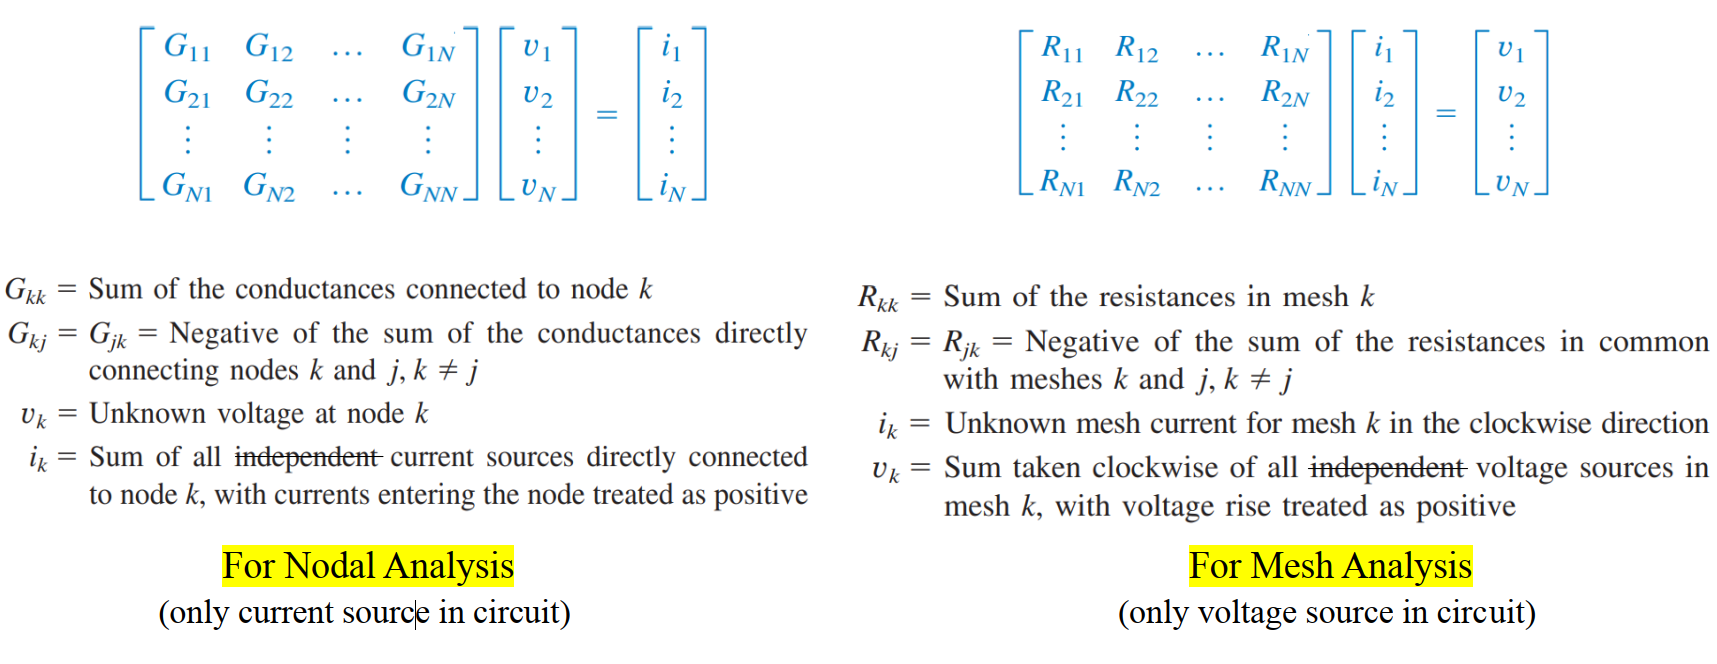
\includegraphics[width=1\textwidth]{ycy/Analysis/analysis.png}
%         \end{figure}
%     \end{frame}
%     %------------------------------------------------
%     \begin{frame}
%     \frametitle{Supernode \& Supermesh}
%     \begin{figure}[H]
%             \centering
%             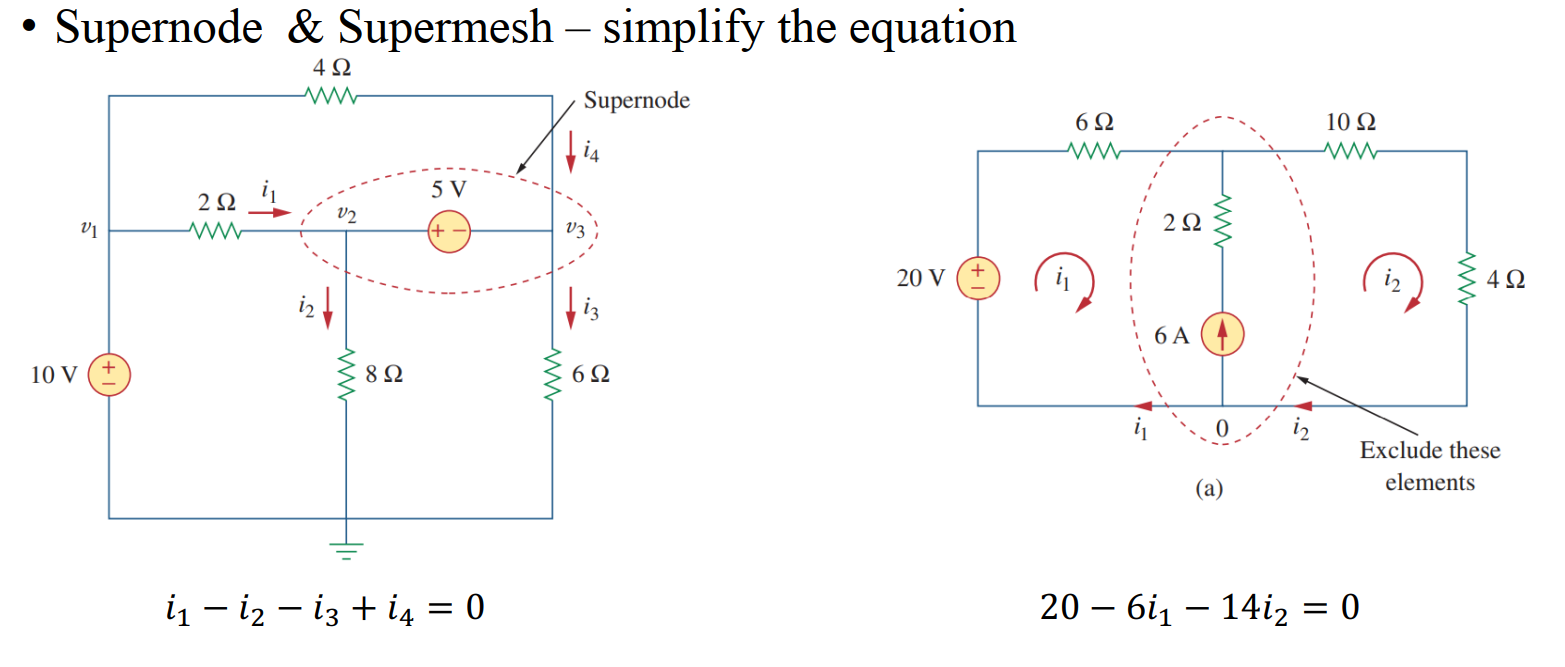
\includegraphics[width=1\textwidth]{ycy/Analysis/super.png}
%         \end{figure}
%     \end{frame}
%     %------------------------------------------------
%     \begin{frame}
%     \frametitle{Exercise}
%     \begin{figure}[H]
%             \centering
%             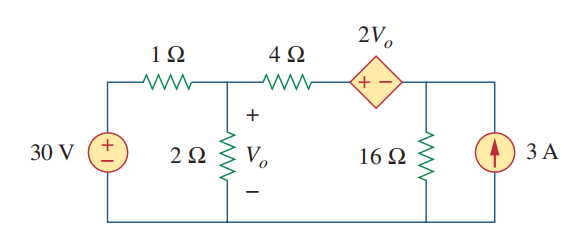
\includegraphics[width=1\textwidth]{ycy/Analysis/exer.png}
%         \end{figure}
%     \end{frame}
    
%     \begin{frame}
%     \frametitle{Exercise}
%     \begin{figure}[H]
%             \centering
%             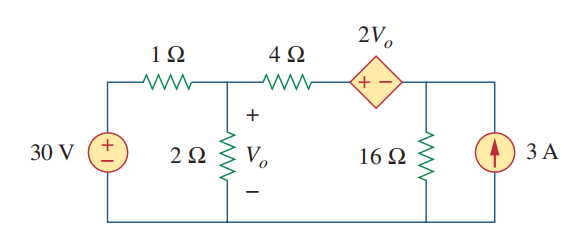
\includegraphics[width=1\textwidth]{ycy/Analysis/exer.png}
%         \end{figure}
%     \centerline{\textbf{Answer:} $\frac{648}{29} V \approx 22.34V$ }
%     \end{frame}


% %%%%%%%%%%%%%%%%%%%%%%%%%%%%%%%%%%%%%%%%%%%%%%%%%%%
% % CIRCUIT THEOREMS
% \section{Circuit Theorems}

%     \begin{frame}{Overview-Chapter4 Circuit Theorems}
%     \begin{itemize}
%     \item Linearity Property
%     \newline
%     \item Superposition
%     \newline
%     \item Source Transformation
%     \newline
%     \item Thevenin's Theorem
%     \newline
%     \item Norton's Theorem
%     \newline
%     \item Maximum Power Transfer
%     \end{itemize}
%     \end{frame}
    
%     %%%%%%%%%%%%%%%%%%%%%%%%%%%%%
    
%     \begin{frame}{Linearity Property}
%     homogeneous: if $x\rightarrow y$, then $kx\rightarrow ky$
%     \newline
%     additive: if $x_1\rightarrow y_1$ and $x_2\rightarrow y_2$, then $x_1+x_2\rightarrow y_1+y_2$
%     \newline
%     linear circuit: homogeneous and additive
%     \newline
%     \textbf{Exercise}
%     \begin{figure}
%     \centering
%     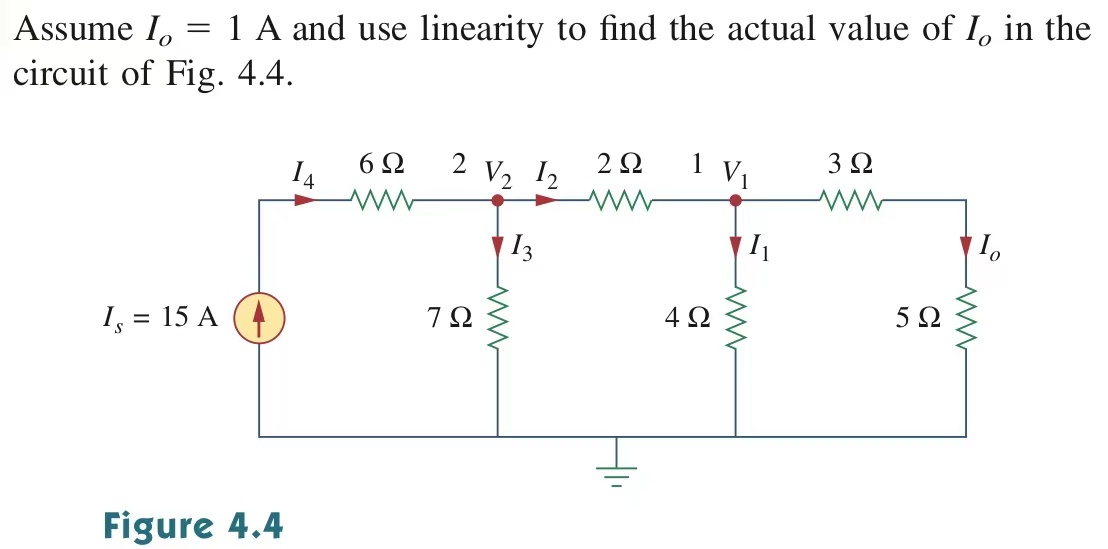
\includegraphics[scale=0.2]{ycy/Cir/1.jpg}
%     \end{figure}
%     \end{frame}
    
%     %%%%%%%%%%%%%%%%%%%%%%%%%%%%%
    
%     \begin{frame}{Exercise}
%     \begin{figure}
%     \centering
%     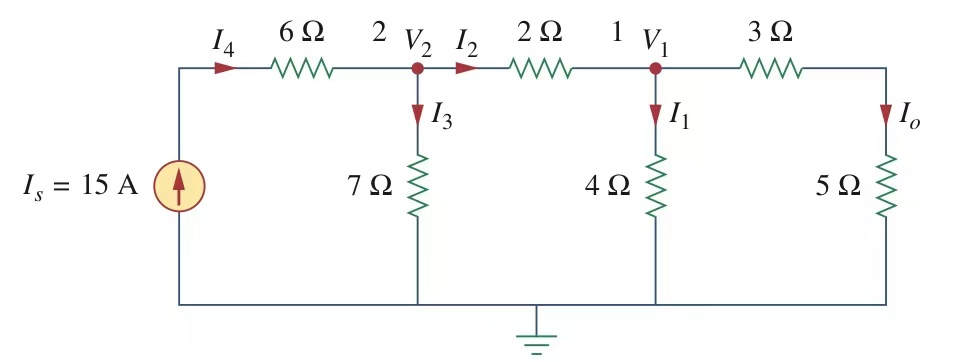
\includegraphics[scale=0.2]{ycy/Cir/2.jpg}
%     \end{figure}
%     \textbf{Answer:} $I_0=3A$
%     \end{frame}
    
%     %%%%%%%%%%%%%%%%%%%%%%%%%%%%%
    
%     \begin{frame}{Superposition}
%     \textbf{Steps}
%     \newline
%     \begin{enumerate}
%     \item Only consider one \textbf{independent} source.
%     \begin{itemize}
%     \item voltage source: short circuit
%     \item current source: open circuit
%     \newline
%     \end{itemize}
%     \item Use additivity.
%     \end{enumerate}
%     \end{frame}
    
%     %%%%%%%%%%%%%%%%%%%%%%%%%%%%%
    
%     \begin{frame}{Exercise}
%     Find $i$ in the circuit.
%     \begin{figure}
%     \centering
%     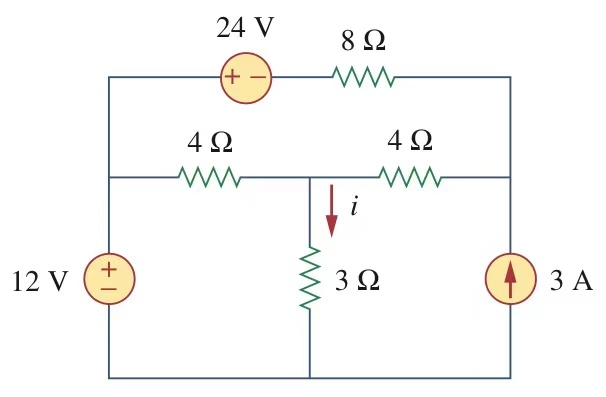
\includegraphics[scale=0.4]{ycy/Cir/4.jpg}
%     \end{figure}
%     \end{frame}
    
%     %%%%%%%%%%%%%%%%%%%%%%%%%%%%%
    
%     \begin{frame}{Source Transformation}
%     We can replace a voltage source with a resistance with a
%     corresponding current source with the same resistance to simplify the circuit. 
%     \newline
%     In the case shown below, $v_s=i_s\times R$
%     \begin{figure}
%     \centering
%     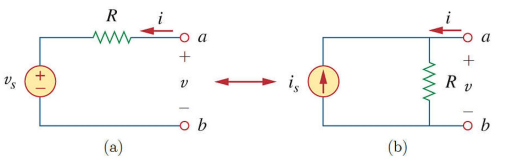
\includegraphics[scale=0.8]{ycy/Cir/5.png}
%     \end{figure}
%     For dependent sources, the source transformation is also valid.
    
%     \end{frame}
    
%     %%%%%%%%%%%%%%%%%%%%%%%%%%%%%
    
%     \begin{frame}{Thevenin’s Theorem}
%     A linear two-terminal circuit can be replaced by an equivalent circuit consisting of a voltage source $V_{Th}$ in series with a resistor $R_{Th}$.
    
%     \begin{figure}
%     \centering
%     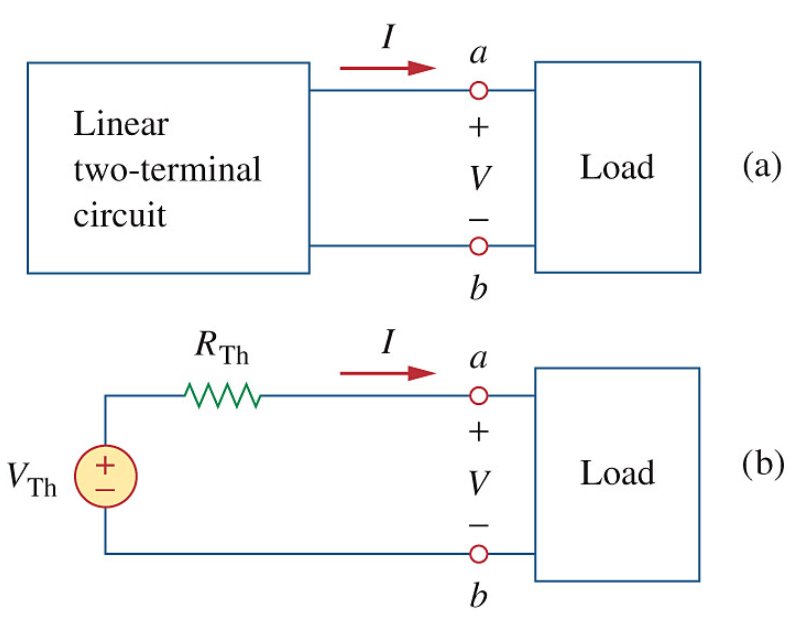
\includegraphics[scale=0.3]{ycy/Cir/7.png}
%     \end{figure}
    
%     \begin{itemize}
%     \item $V_{Th}$: the open-circuit voltage at the terminals.
%     \item $R_{Th}$: the equivalent resistance at the terminals when all the \textcolor{red}{independent sources} are turned off.
%     \end{itemize}
%     \end{frame}
    
%     %%%%%%%%%%%%%%%%%%%%%%%%%%%%%
    
%     \begin{frame}{Norton’s Theorem}
%     A linear two-terminal circuit can be replaced by an equivalent circuit consisting of a current source $I_{Th}$ in parallel with a resistor $R_{Th}$.
    
%     \begin{figure}
%     \centering
%     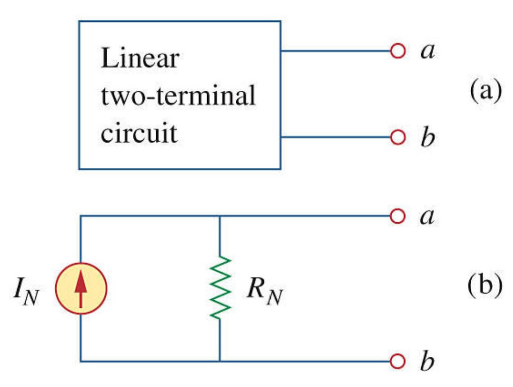
\includegraphics[scale=0.3]{ycy/Cir/9.png}
%     \end{figure}
    
%     \begin{itemize}
%     \item $I_{Th}$: the short-circuit current at the terminals.
%     \item $R_{Th}$: the equivalent resistance at the terminals when all the \textcolor{red}{independent sources} are turned off.
%     \end{itemize}
%     \end{frame}
    
%     %%%%%%%%%%%%%%%%%%%%%%%%%%%%%
    
%     \begin{frame}{Maximum Power Transfer}
    
%     A circuit is usually designed to provide power to a load. For different kinds of circuits, we have different concerns
    
%     \begin{itemize}
%         \item \textbf{Maximum Power Efficiency:}
%         In power utility systems, the amount of electricity is very large. Therefore, how to \textcolor{red}{ increase the efficiency of power transfer} becomes an important problem.
%         \item \textbf{Maximum Power Transfer:}  In communication and instrumental systems, the amount of electricity is small so the problem of efficiency is not so important. Instead, we want to \textcolor{red}{transfer as much of power as possible to the load}.
%     \end{itemize}.
    
    
%     \end{frame}
    
%     %%%%%%%%%%%%%%%%%%%%%%%%%%%%%
    
%     \begin{frame}{Maximum Power Transfer}
     
%     The Thevenin’s equivalent circuit is useful in finding the maximum power delivered to a load. In the circuit below, $R_L$ represents the load.
    
    
%     \begin{figure}
%     \centering
%     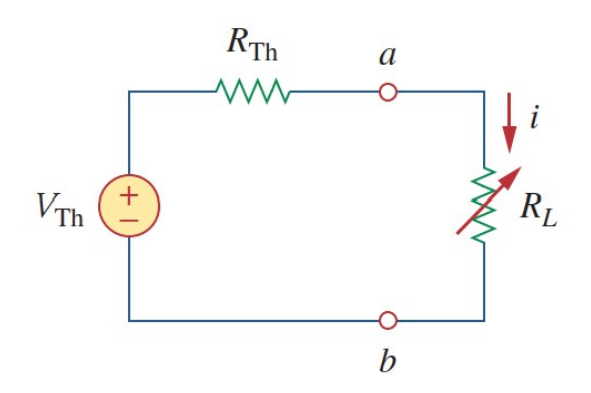
\includegraphics[scale=0.5]{ycy/Cir/11.png}
%     \end{figure}
    
%     \end{frame}
    
%     %%%%%%%%%%%%%%%%%%%%%%%%%%%%%
    
%     \begin{frame}{Maximum Power Theorem}
    
%     Since
%     $$
%         p=i^2R_{L}=\Big(\frac{V_{Th}}{R_{Th}+R_L}\Big)^2 R_{L} 
%     $$
%     Let $\frac{dP}{dR_L}=V_{Th}^2\frac{R_{Th}-R_L}{(R_{Th}+R_L)^3}=0$, we have $R_L=R_{Th}$.
    
%     And when $R_{L}=R_{Th}$, $\frac{d^2P}{dR_L^2}=V_{Th}^2\frac{2R_l-4R_{Th}}{(R_{Th}+R_L)^4}=-\frac{V_{Th}^2}{8R_{Th}^2}<0$.
    
%     Thus $p$ reaches maximum at $R_L=R_{Th}$. \textcolor{}{$p_{max}=\frac{V_{Th}^2}{4R_{Th}}$}
    
%     \end{frame}
    

% %%%%%%%%%%%%%%%%%%%%%%%%%%%%%%%%%%%%%%%%%%%%%%%%%%%
% % OP-AMP
% \section{Operational Amplifiers}
    


  
    
%     %%%%%%%%%%%%%%%%%%%%%%%%%%%%%
%     \begin{frame}{Ideal Op-amp}
    
%     Assumption:
%     \begin{itemize}
%         \item Infinite open-loop gain ($A = \infty$)
%         \item Infinite input resistance ($R_i = \infty$)
%         \item Zero output resistance ($R_0 = 0$)
%         \item (Does not mean that $v_0 = \infty$)
%     \end{itemize}
    
%     \begin{multicols}{2}
%         \sectiont{}
%         \begin{figure}[H]
%             \centering
%             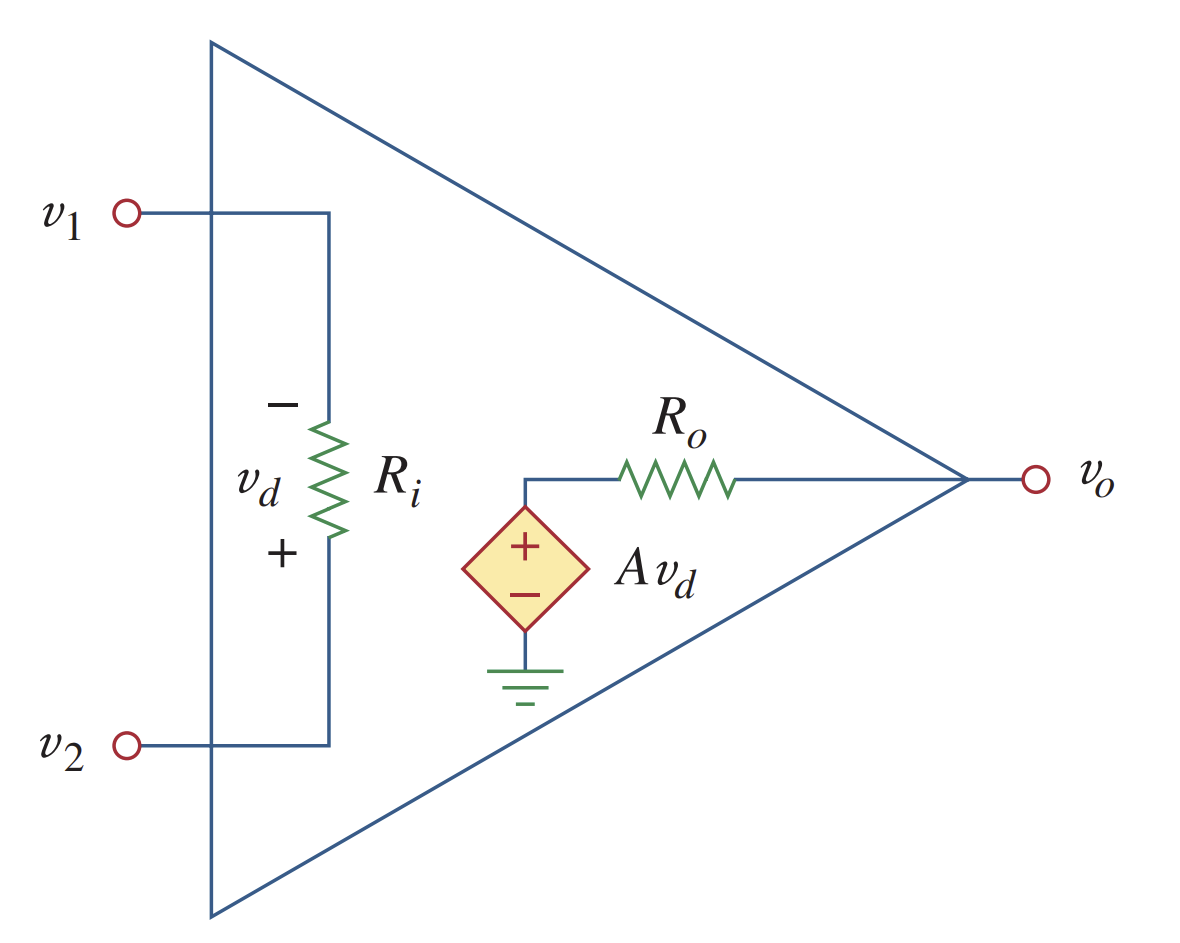
\includegraphics[width=0.35\textwidth]{img_opamp/3_opamp equivalent.png}
%             \caption{Op-amp's equivalent circuit}
%         \end{figure}
%         \sectiont{}
%         \begin{figure}[H]
%             \centering
%             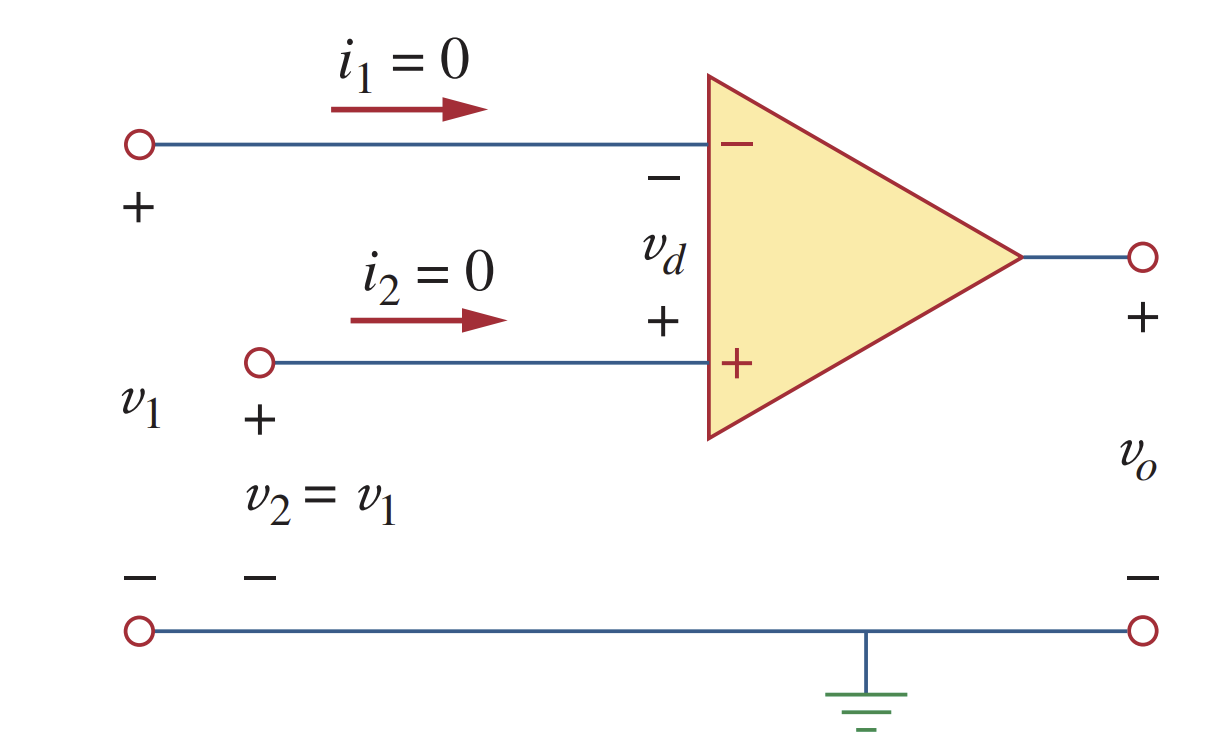
\includegraphics[width=0.46\textwidth]{img_opamp/4_ideal op amp.png}
%             \caption{Symbol of ideal op-amp}
%         \end{figure}
        
%     \end{multicols}
    
        
%     \end{frame}
    
%     %%%%%%%%%%%%%%%%%%%%%%%%%%%%%
%     \begin{frame}{Ideal Op-amp}
    
%     Characteristics of ideal op-amp:
%     \begin{itemize}
%         \item Open circuit at two input terminals ($i_1 = i_2 = 0$)
%         \item Same voltage at two input terminals ($v_1 = v_2$)
%         \item (\textbf{Does not mean that $i_o = 0$!})
%     \end{itemize}
    
%     \begin{multicols}{2}
%         \sectiont{}
%         \begin{figure}[H]
%             \centering
%             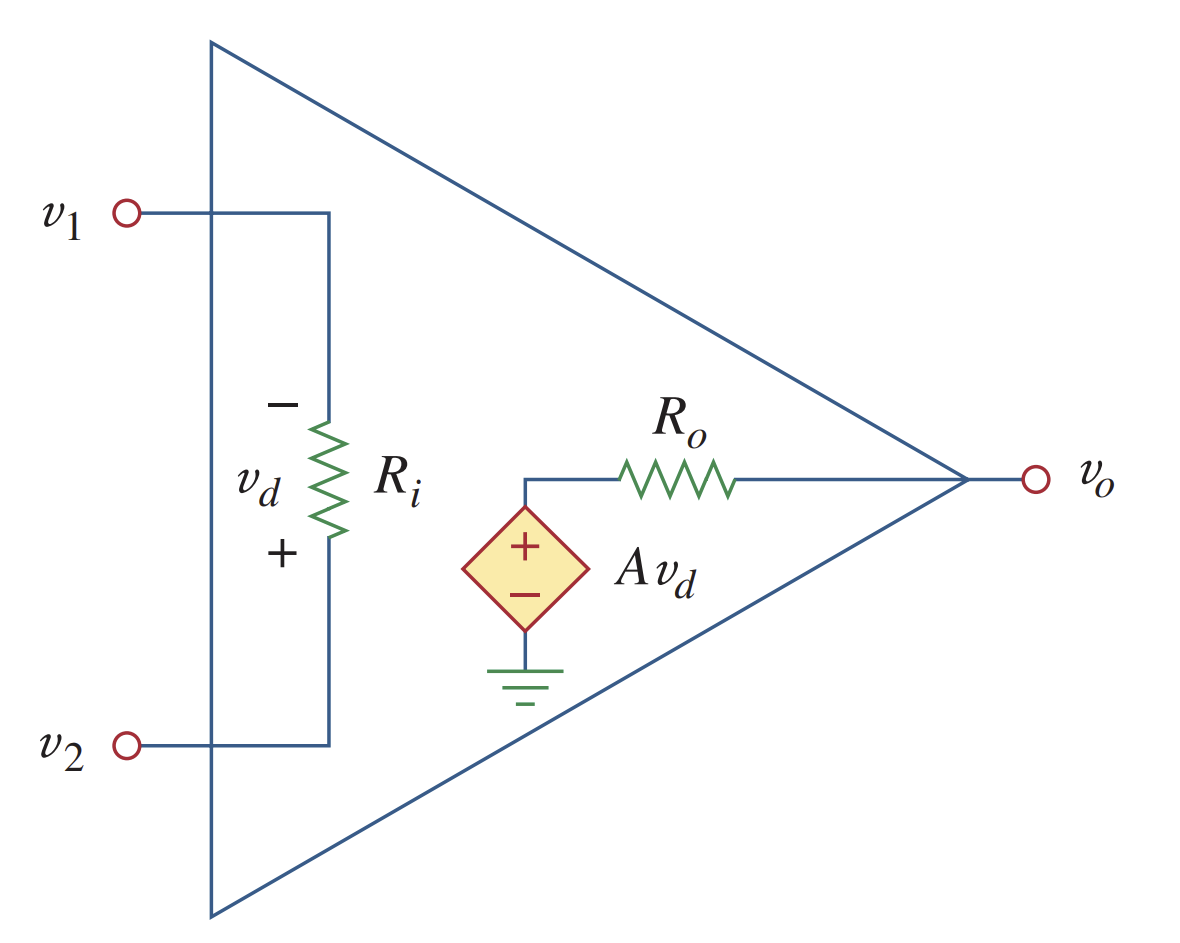
\includegraphics[width=0.35\textwidth]{img_opamp/3_opamp equivalent.png}
%             \caption{Op-amp's equivalent circuit}
%         \end{figure}
%         \sectiont{}
%         \begin{figure}[H]
%             \centering
%             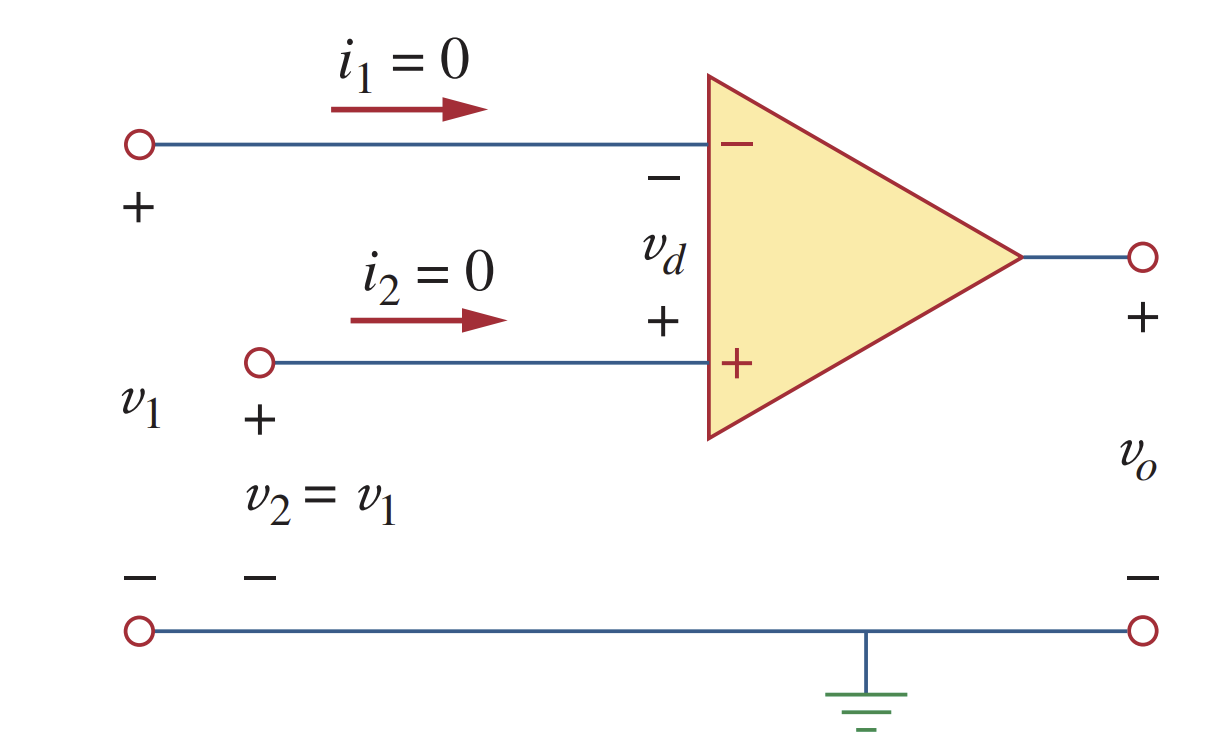
\includegraphics[width=0.46\textwidth]{img_opamp/4_ideal op amp.png}
%             \caption{Symbol of ideal op-amp}
%         \end{figure}
        
%     \end{multicols}
        
%     \end{frame}
    
%     %%%%%%%%%%%%%%%%%%%%%%%%%%%%%
%     \begin{frame}{Basic Op-amp Circuits: Summary}
%     For basic op-amp circuits:
%     \begin{table}[]
%         \centering
%         \begin{tabular}{cc}
%             \toprule
%             Op-amp circuits & Input-output relationship\\
%             \midrule
%             Inverting amplifier & $A = \frac{v_0}{v_i} = -\frac{R_f}{R_1}$\\
%             Non-inverting amplifier & $A = \frac{v_0}{v_i} = 1 + \frac{R_f}{R_1}$\\
%             Voltage follower & $v_o=v_i$\\
%             Summing amplifier & $v_o = -(\frac{R_f}{R_1}v_1 + \frac{R_f}{R_2}v_2 + \frac{R_f}{R_3}v_3)$\\
%             Difference amplifier & $v_o = \left[ (\frac{R_2}{R_1}+1)(\frac{R_4/R_3}{1+R_4/R_3})\right]v_2 - \left[\frac{R_2}{R_1}\right]v_1$\\
%             \bottomrule
%         \end{tabular}
%     \end{table}
    
%     For complicated op-amp circuits:
%     \begin{itemize}
%         \item Identify basic op-amp circuits within it
%         \item Use the formula for cascaded op-amp circuit
%         \item Be proficient in listing nodal analysis equations to obtain $v_o/v_i$
%     \end{itemize}
        
%     \end{frame}
    

%%%%%%%%%%%%%%%%%%%%%%%%%%%%%%%%%%%%%%%%%%%%%%%%%%%
% CAPACITORS AND INDUCTORS
\section{Capacitors and Inductors}


    \begin{frame}{Capacitors}
    \begin{enumerate}
        \item \textbf{Open Circuit Property} When the voltage across a capacitor is not changing with time (\textbf{DC steady state}), \textbf{the capacitor could be treated as an open circuit}.
        \item \textbf{Continuity property} The voltage on a capacitor must be continuous. 
        \begin{figure}
        \centering
        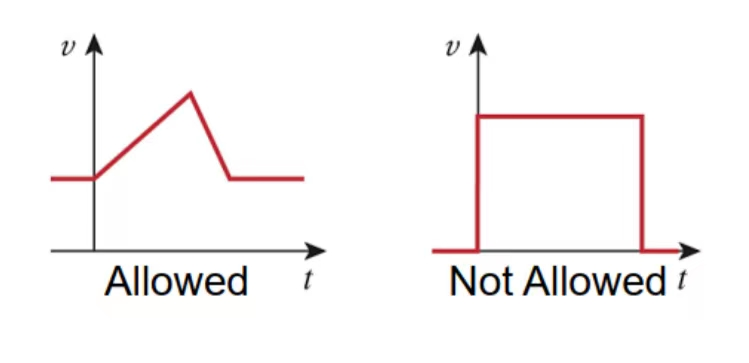
\includegraphics[width=2in]{ycy/Chap6/f1.jpg}
        \end{figure}
        \item \textbf{Capacitors IV relationship} 
        \begin{equation*}
            i=C\frac{dv}{dt}
        \end{equation*}
        property 2 can be intuitively shown be property 3. If the voltage across the capacitor is not continuous, say $\frac{dv}{dt}=\infty$, which will cause $i$ to be infinity.
    \end{enumerate}
    \end{frame}
    
    \begin{frame}{Capacitors}
    \begin{enumerate}
        \item \textbf{An ideal capacitor will not dissipate energy.} It takes power from the circuit when storing energy in its electric field and returns previously stored energy when delivering power to the circuit.
        \item \textbf{A real capacitor has a large leakage resistance} 
        \begin{figure}
        \centering
        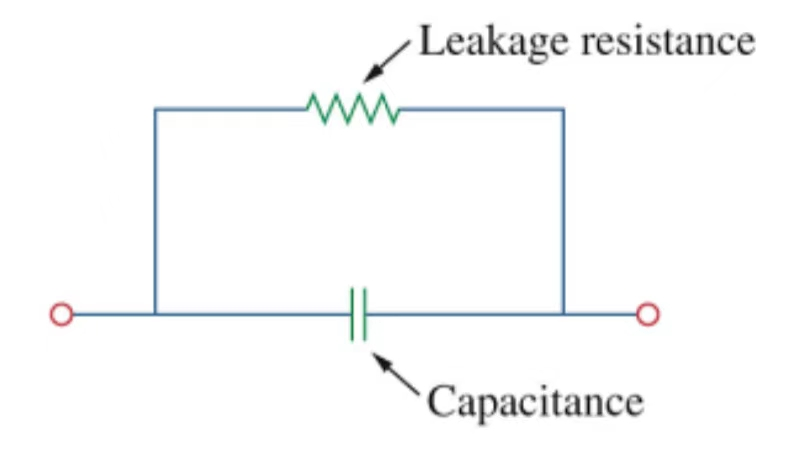
\includegraphics[width=2in]{ycy/Chap6/f2.jpg}
        \end{figure}
    
    \end{enumerate}
    \end{frame}
    
    \begin{frame}{Capacitors in parallel $\&$ in series}
    \begin{itemize}
        \item \textbf{capacitors in parallel}
        \begin{figure}
        \centering
        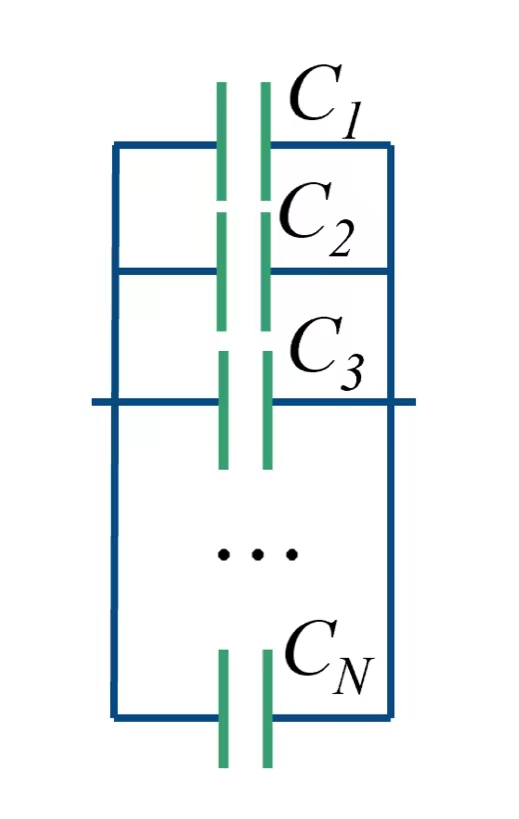
\includegraphics[width=0.5in]{ycy/Chap6/f3.jpg}
        \end{figure}
        \begin{equation*}
            C_{eq}=C_1+C_2+C_3+...+C_N
        \end{equation*}
        
        \item \textbf{capacitors in series}
        \begin{figure}
        \centering
        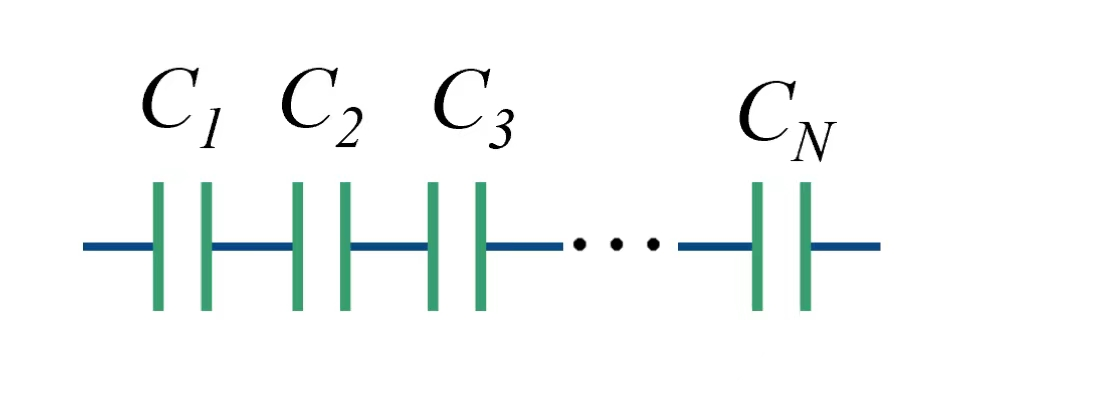
\includegraphics[width=1.2in]{ycy/Chap6/f4.jpg}
        \end{figure}
        \begin{equation*}
            \frac{1}{C_{eq}}=\frac{1}{C_1}+\frac{1}{C_2}+\frac{1}{C_3}+\frac{1}{C_4}+...+\frac{1}{C_N}
        \end{equation*}
        \end{itemize}
    \end{frame}
    
    \begin{frame}{Energy stored in Capacitors}
    \textbf{The instantaneous power} delivered to the capacitor is 
        \begin{equation*}
            p=vi=v(C\frac{dv}{dt})
        \end{equation*}
        Therefore, \textbf{the total energy} stored in the capacitor is 
        \begin{equation*}
            w=\frac{1}{2}CV^2
        \end{equation*}
    \end{frame}
    
    \begin{frame}{Inductors}
    \begin{enumerate}
        \item \textbf{Short Circuit Property} When the current through an inductor is not changing with time (\textbf{DC steady state}), \textbf{the inductor could be treated as a short circuit in the circuit}.
        \item \textbf{Continuity property} The current through a capacitor must be continuous. 
        \item \textbf{Inductor IV relationship} 
        \begin{equation*}
            v=L\frac{di}{dt}
        \end{equation*}
    \end{enumerate}
    \end{frame}
    
    \begin{frame}{Inductors}
    \begin{enumerate}
        \item \textbf{An ideal inductor will not dissipate energy.} It takes power from the circuit when storing energy in its magnetic field and returns previously stored energy when delivering power to the circuit.
        \item \textbf{A real inductor has a significant winding resistance and a small winding capacitance} 
        \begin{figure}
        \centering
        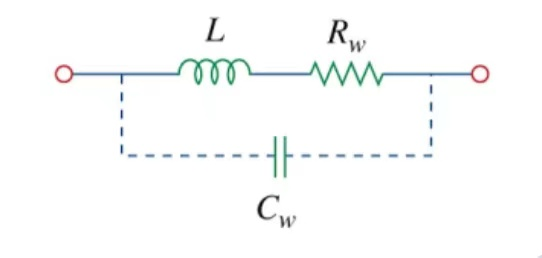
\includegraphics[width=2in]{ycy/Chap6/f5.jpg}
        \end{figure}
    
    \end{enumerate}
    \end{frame}
    
    \begin{frame}{Inductors in parallel $\&$ in series}
    \begin{itemize}
        \item \textbf{inductors in parallel}
        \begin{figure}
        \centering
        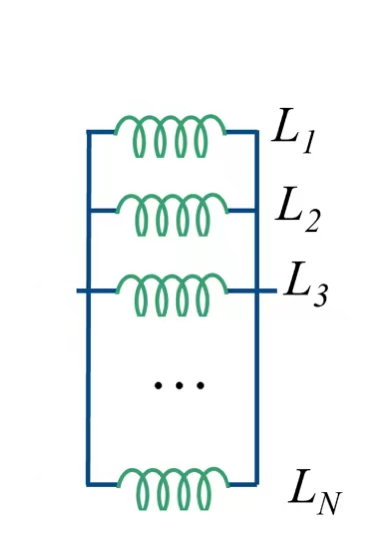
\includegraphics[width=0.7in]{ycy/Chap6/f6.jpg}
        \end{figure}
        \begin{equation*}
            \frac{1}{L_{eq}}=\frac{1}{L_1}+\frac{1}{L_2}+\frac{1}{L_3}+\frac{1}{L_4}+...+\frac{1}{L_N}
        \end{equation*}
        
        \item \textbf{inductors in series}
        \begin{figure}
        \centering
        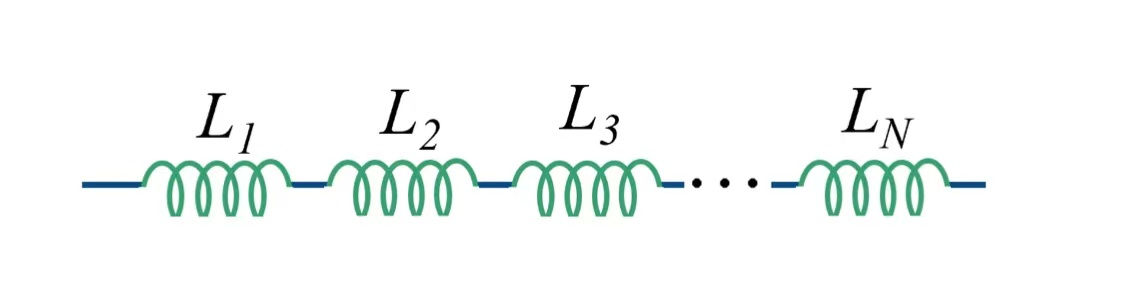
\includegraphics[width=1.4in]{ycy/Chap6/f7.jpg}
        \end{figure}
        \begin{equation*}
            L_{eq}=L_1+L_2+L_3+L_4+...+L_N
        \end{equation*}
        \end{itemize}
    \end{frame}
    \begin{frame}{Energy stored in Inductors}
    \textbf{The instantaneous power} delivered to the inductor is 
        \begin{equation*}
            p=vi=(L\frac{di}{dt})i
        \end{equation*}
        Therefore, \textbf{the total energy} stored in the inductor is 
        \begin{equation*}
            w=\frac{1}{2}Li^2
        \end{equation*}
    \end{frame}
    
    \begin{frame}{Summary of Capacitors and Inductors}
        \begin{figure}
        \centering
        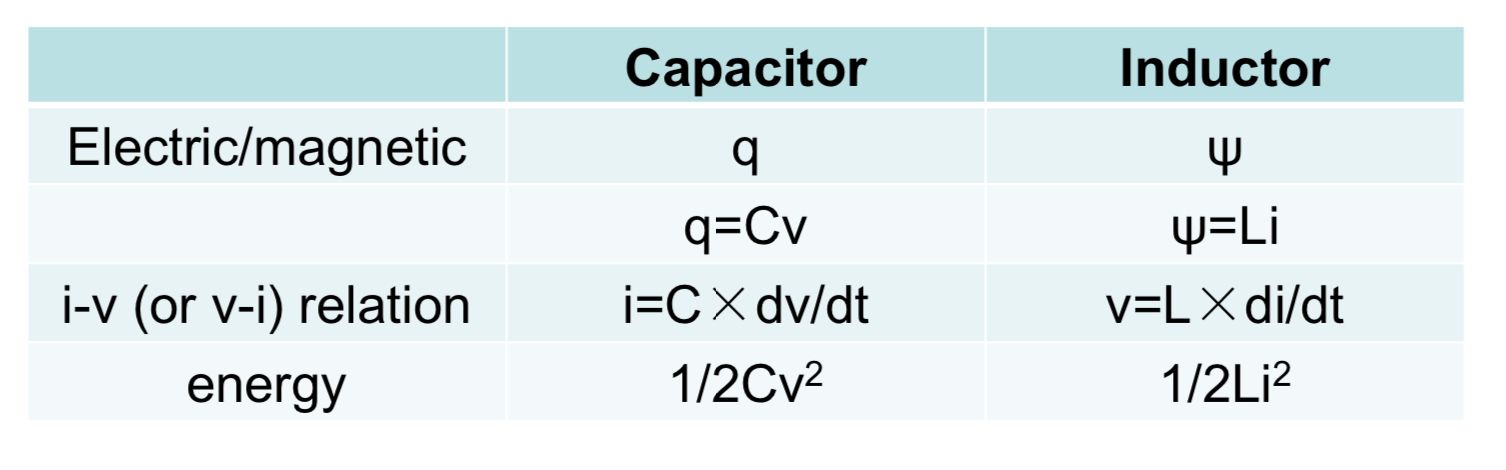
\includegraphics[width=3in]{ycy/Chap6/f8.jpg}
        \end{figure}
        \begin{figure}
        \centering
        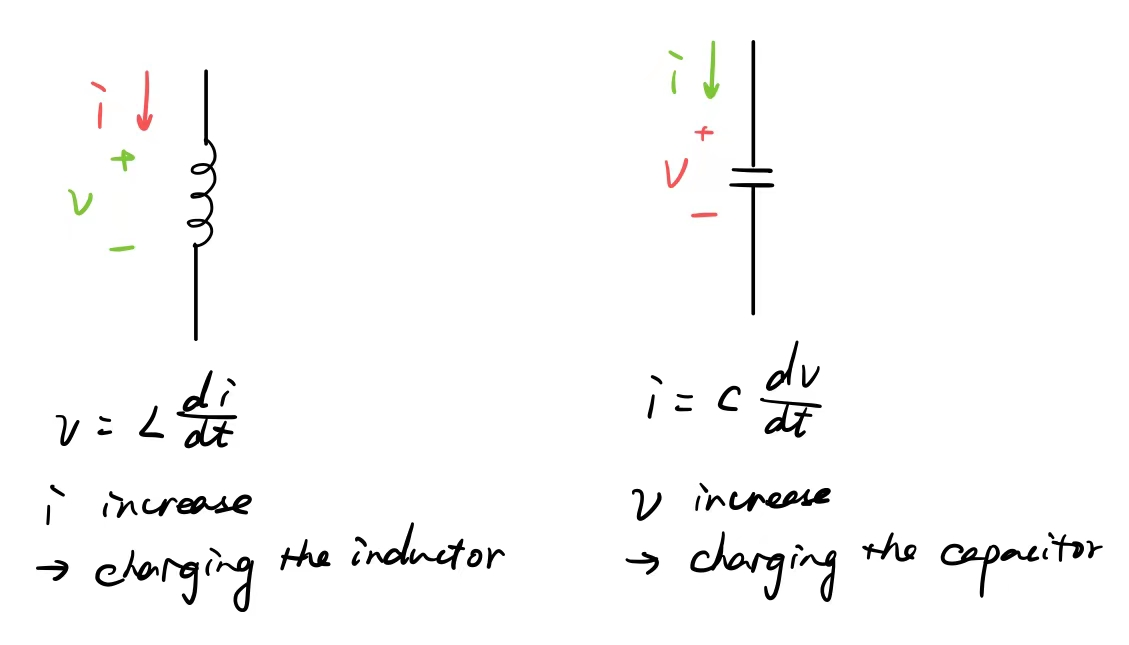
\includegraphics[width=3in]{ycy/Chap6/f9.jpg}
        \end{figure}
    \end{frame}

%%%%%%%%%%%%%%%%%%%%%%%%%%%%%%%%%%%%%%%%%%%%%%%%%%%
% 1ST-ORDER CIRCUITS
\section{First-Order Circuit}
% \subsection{First-order Circuit}

%%%%%%%%%%%%%%%%%%%%%%%%%%%%%
\begin{frame}{Introduction}

Definition: a first-order circuit is a circuit that contains \textbf{only} \textbf{ONE} capacitor/inductor after circuit simplification.

Motivation: we want to investigate how the circuit responses if we
    \begin{itemize}
        \item Store energy to capacitor/inductor
        \item Let the capacitor/inductor releases energy
    \end{itemize}

\begin{table}[]
    \centering
    \begin{tabular}{c|cc}
        \hline
        & Only one Capacitor & Only one inductor \\
        \hline
        Store energy &Step input RC& Step input RL \\
         % \hline
        Release energy &Source free RC& Source free RL\\
         \hline
    \end{tabular}
    % \caption{Caption}
    % \label{tab:my_label}
\end{table}


\end{frame}


%%%%%%%%%%%%%%%%%%%%%%%%%%%%%

\begin{frame}{Singularity Functions}

\begin{table}[]
    \centering
    \begin{small}
        
    \begin{tabular}{ccc}
        \toprule
        \textbf{Unit ramp} & \textbf{Unit step} & \textbf{Unit impulse} \\
         \midrule
         $$ r(t)=
        \begin{cases}
        0, t \leq 0\\
        t, t>0
        \end{cases} $$
         &
         $$ u(t)=
        \begin{cases}
        0, t \leq 0\\
        1, t>0
        \end{cases} $$
         &
         $$\delta(t)=
        \begin{cases}
        0, t\neq 0\\
        \text{Undef.}, t=0
        \end{cases}$$
         \\
         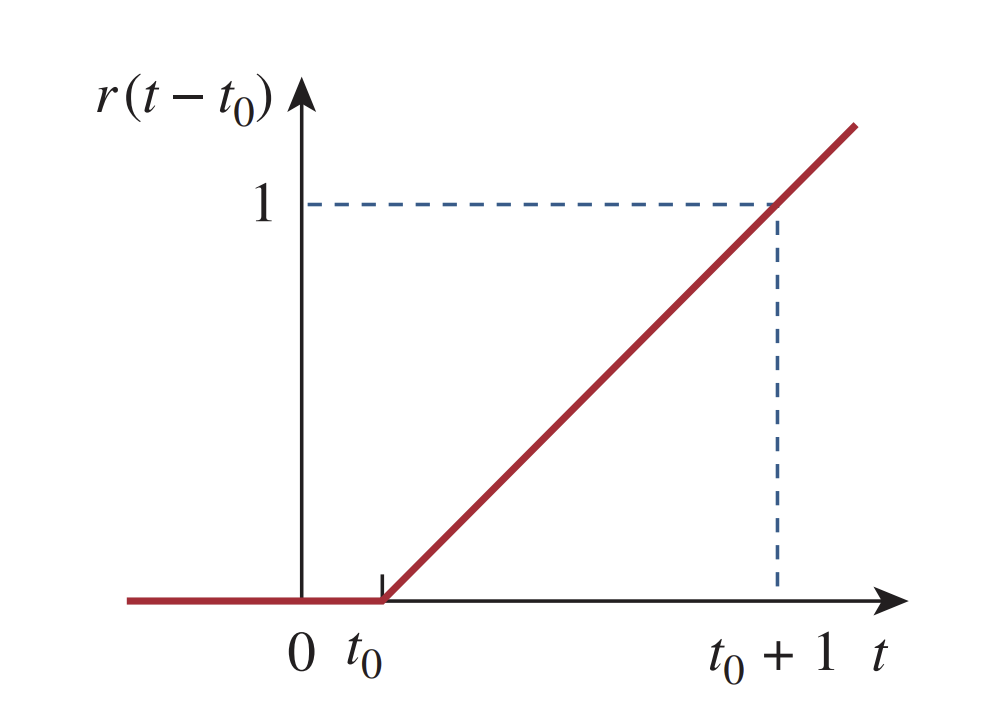
\includegraphics[width=0.3\textwidth]{img_1order/5_rampt.png}
         &
        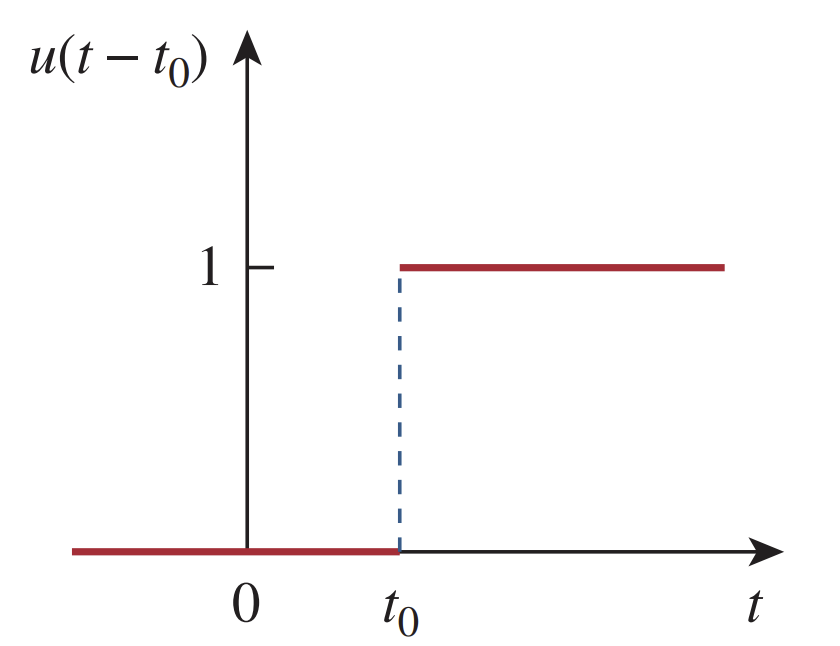
\includegraphics[width=0.3\textwidth]{img_1order/6_ut.png}
         &
         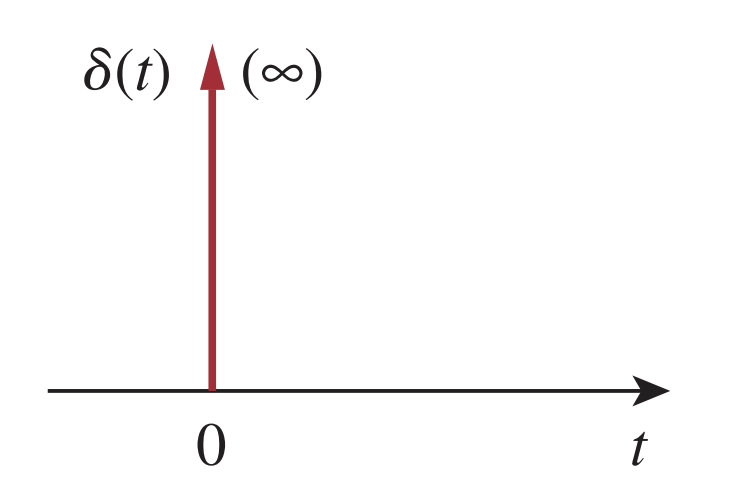
\includegraphics[width=0.29\textwidth]{img_1order/4_deltat.png}
         \\
         \bottomrule
    \end{tabular}
    \end{small}
    % \caption{Caption}
    % \label{tab:my_label}
\end{table}

Give a nice way to represent ``Switch on/off" of the sources/part of circuits.

% Relationships:
$$\delta(t) \stackrel{\int}{\longrightarrow} u(t) \stackrel{\int}{\longrightarrow} r(t)$$


\end{frame}

%%%%%%%%%%%%%%%%%%%%%%%%%%%%%
% \subsection{Source-Free Circuits}
\begin{frame}{Source-Free Circuits (I) Response}


\begin{table}[]
    \centering
    \begin{small}
    \setlength{\tabcolsep}{5mm}
    \begin{tabular}{c|c}
        % \toprule
        \textbf{Source-free RC} & \textbf{Source-free RL}\\
        \begin{figure}
        \centering
        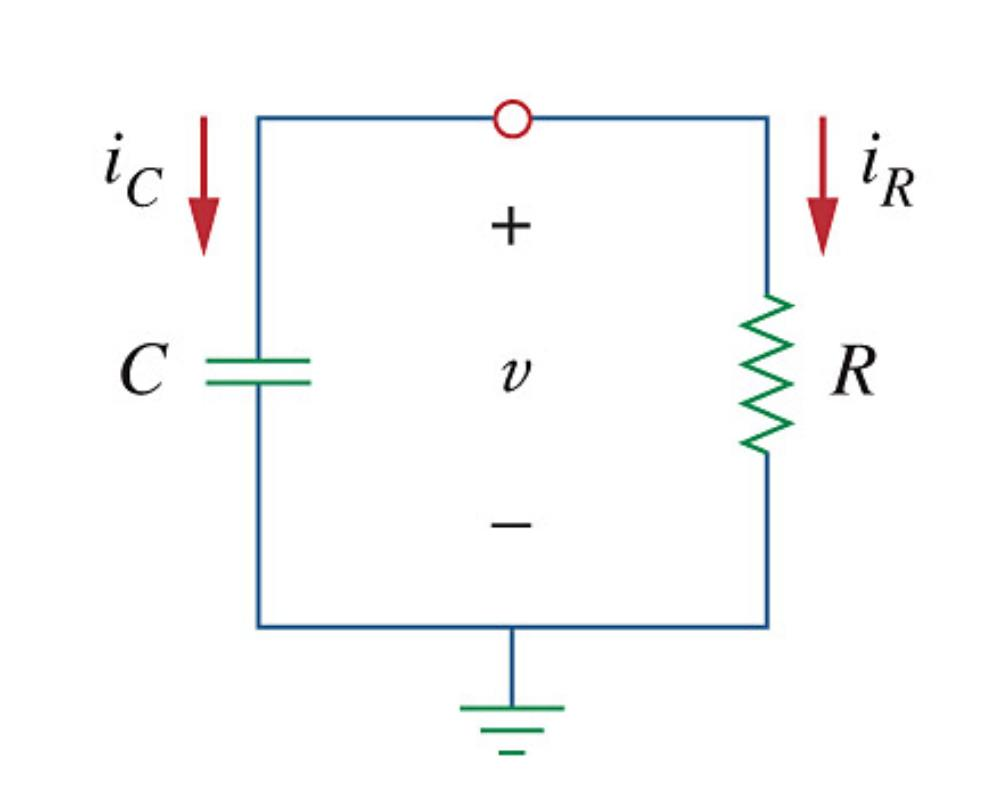
\includegraphics[width=0.35\textwidth]{img_1order/1_source-free_RC.jpg}
        \end{figure}
        &
        \begin{figure}
        \centering
        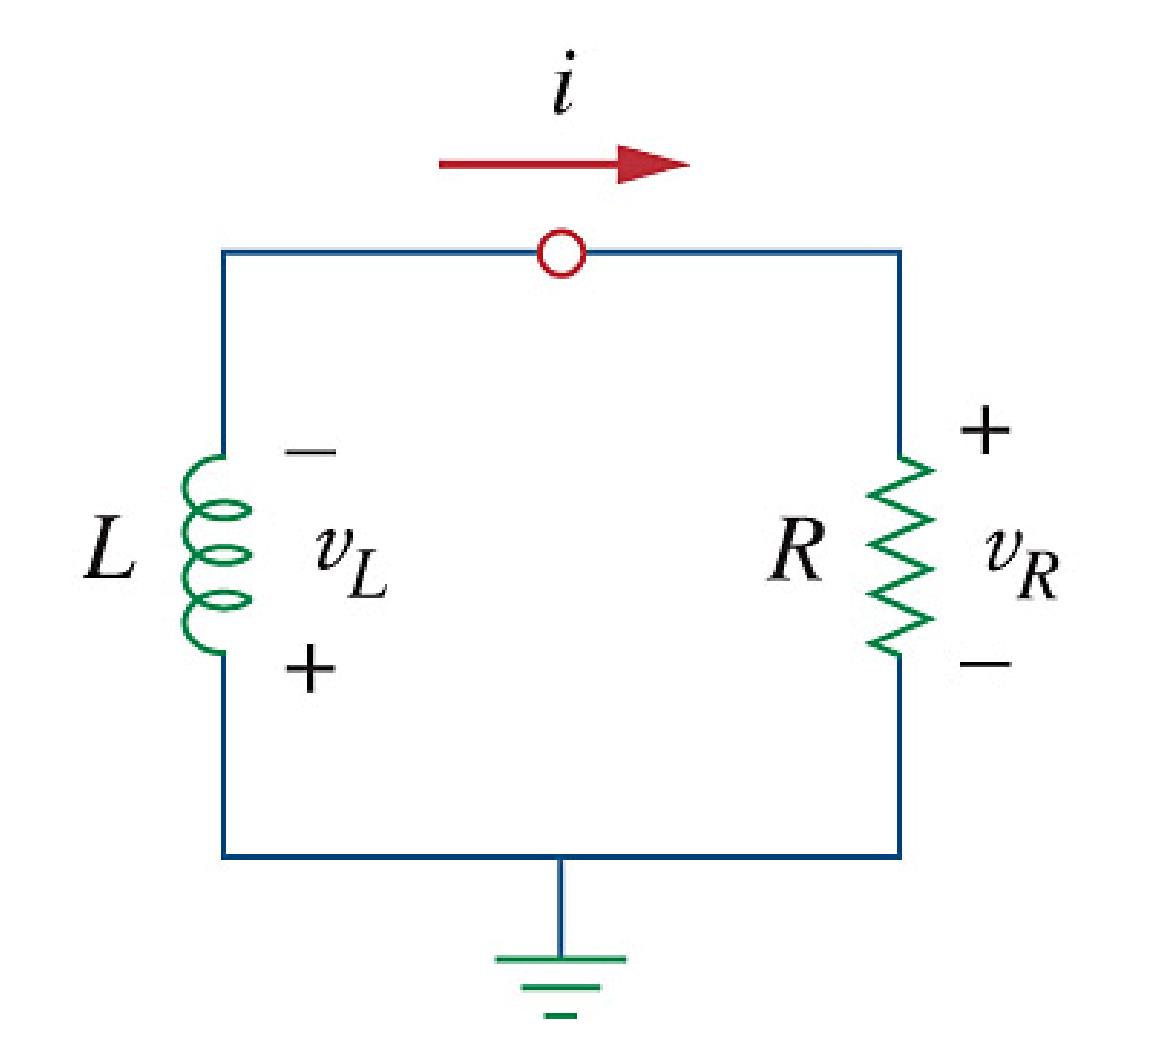
\includegraphics[width=0.35\textwidth]{img_1order/2_source-free_RL.jpg}
        \end{figure}
        \\
        Voltage: $v = v_0 e^{-t/RC}$&Current: $i = i_0 e^{-t/(L/R)}$\\
        &\\
        Time constant: $\tau = RC$&Time constant: $\tau = L/R$\\
        &\\
        Current: $i_R=\frac{v}{R}=\frac{v_0}{R}e^{-t/\tau}$&Voltage: $v_R=iR=\frac{i_0}{R}e^{-t/\tau}$\\
        Power: $p=vi_R=\frac{v_0^2}{R}e^{-2t/\tau}$&Power: $p=v_Ri=i_0^2Re^{-2t/\tau}$\\
        Energy: $w_R = \int_0^tpdt = \frac12Cv_0^2$&Energy: $w_R = \int_0^tpdt = \frac12Li_0^2$\\
        % \bottomrule
    \end{tabular}
    \end{small}
\end{table}



\end{frame}

%%%%%%%%%%%%%%%%%%%%%%%%%%%%%
\begin{frame}{Source-Free Circuits (II) Time Constant}

\begin{figure}
    \centering
    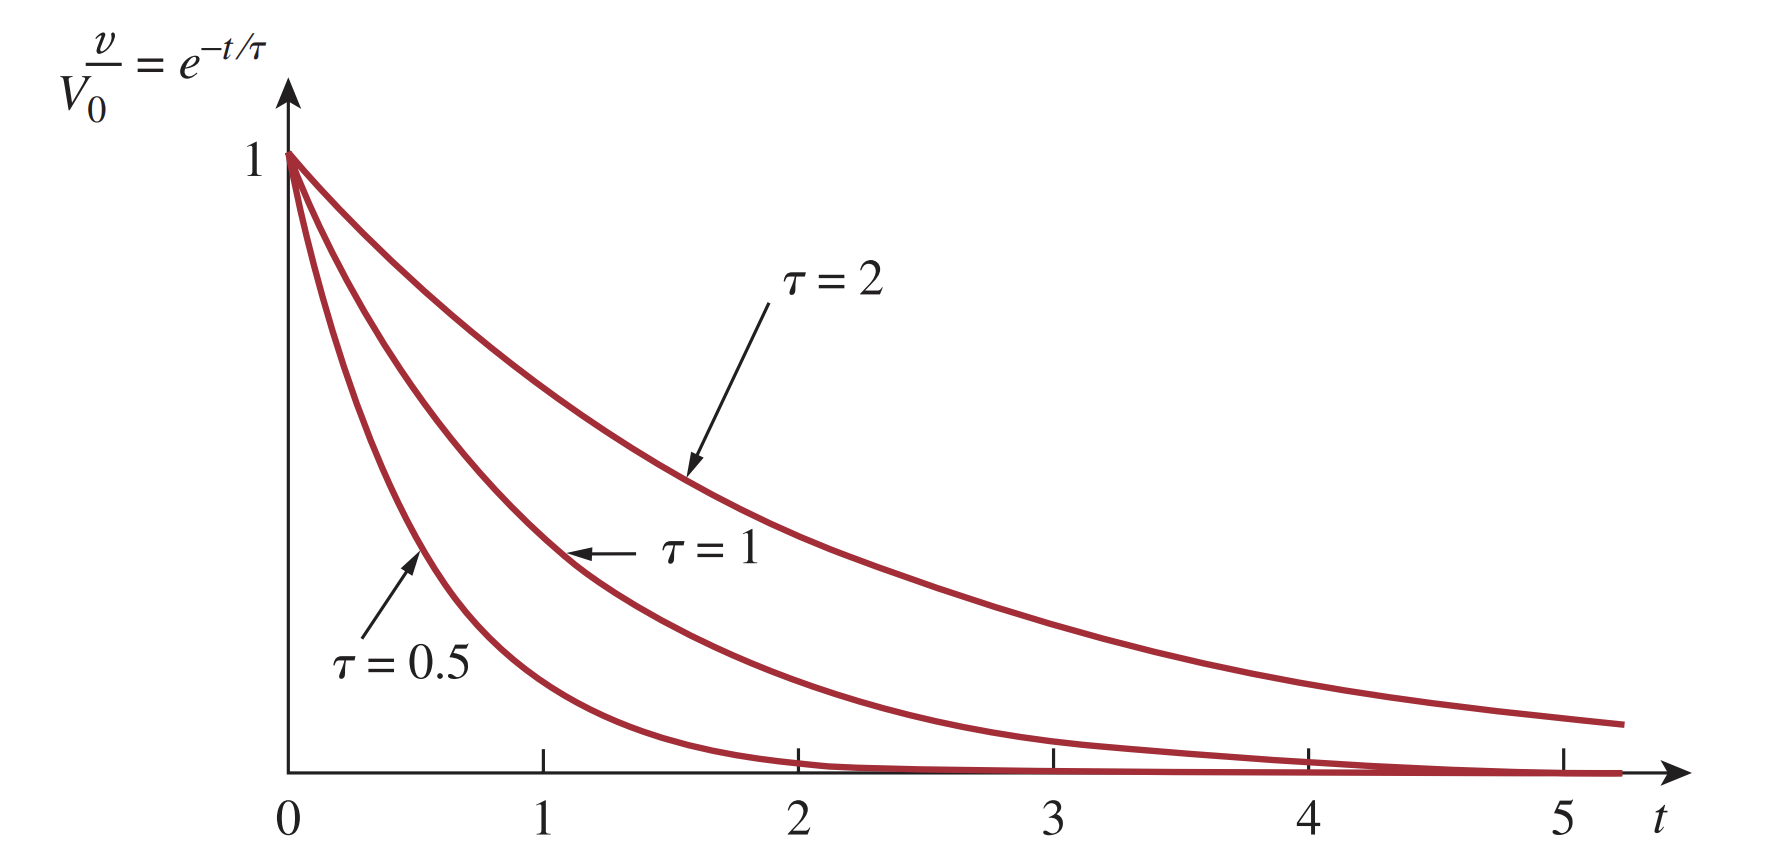
\includegraphics[width=0.7\textwidth]{img_1order/3_plot_response.png}
\end{figure}

\begin{table}[]
    \centering
    \begin{small}
    \begin{tabular}{ccc}
        \toprule
        &Source-free RC & Source-free RL\\
        \midrule
        Time constant&$\tau = RC$&$\tau=L/R$\\
        Relation to initial decay rate&$\frac{d}{dt}(\frac{v}{v_0}) = -1/\tau$&$\frac{d}{dt}(\frac{i}{i_0}) = -1/\tau$\\
        \bottomrule
    \end{tabular}
    \end{small}
\end{table}
\begin{small}

\begin{itemize}
    \item Time required for the response to decay to a factor of $1/e$ or $36.8\%$ of its initial value
    \item Indicates the initial decaying rate
    \item Assume complete decay after $5\tau$
\end{itemize}
\end{small}


\end{frame}

%%%%%%%%%%%%%%%%%%%%%%%%%%%%%
\begin{frame}{Source-Free Circuits (III) General Steps}


\begin{table}[]
    \centering
    % \begin{small}
        
    \begin{tabular}{c|c}
        % \toprule
        \textbf{Source-free RC} & \textbf{Source-free RL}\\
        \begin{figure}
        \centering
        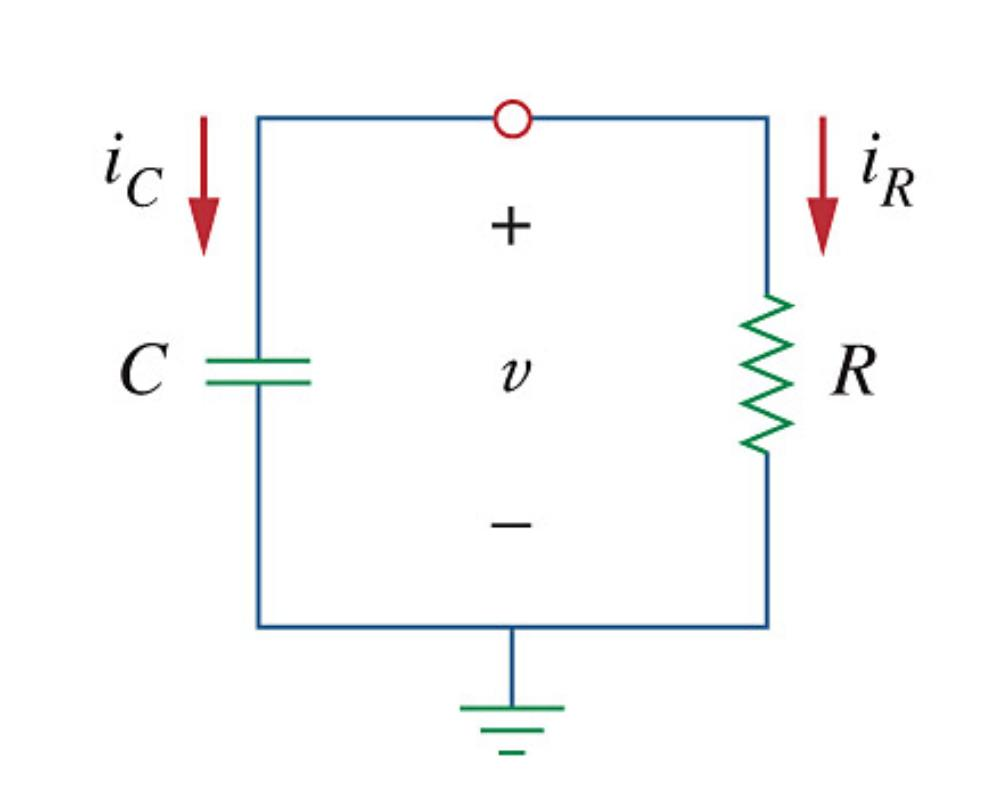
\includegraphics[width=0.35\textwidth]{img_1order/1_source-free_RC.jpg}
        \end{figure}
        &
        \begin{figure}
        \centering
        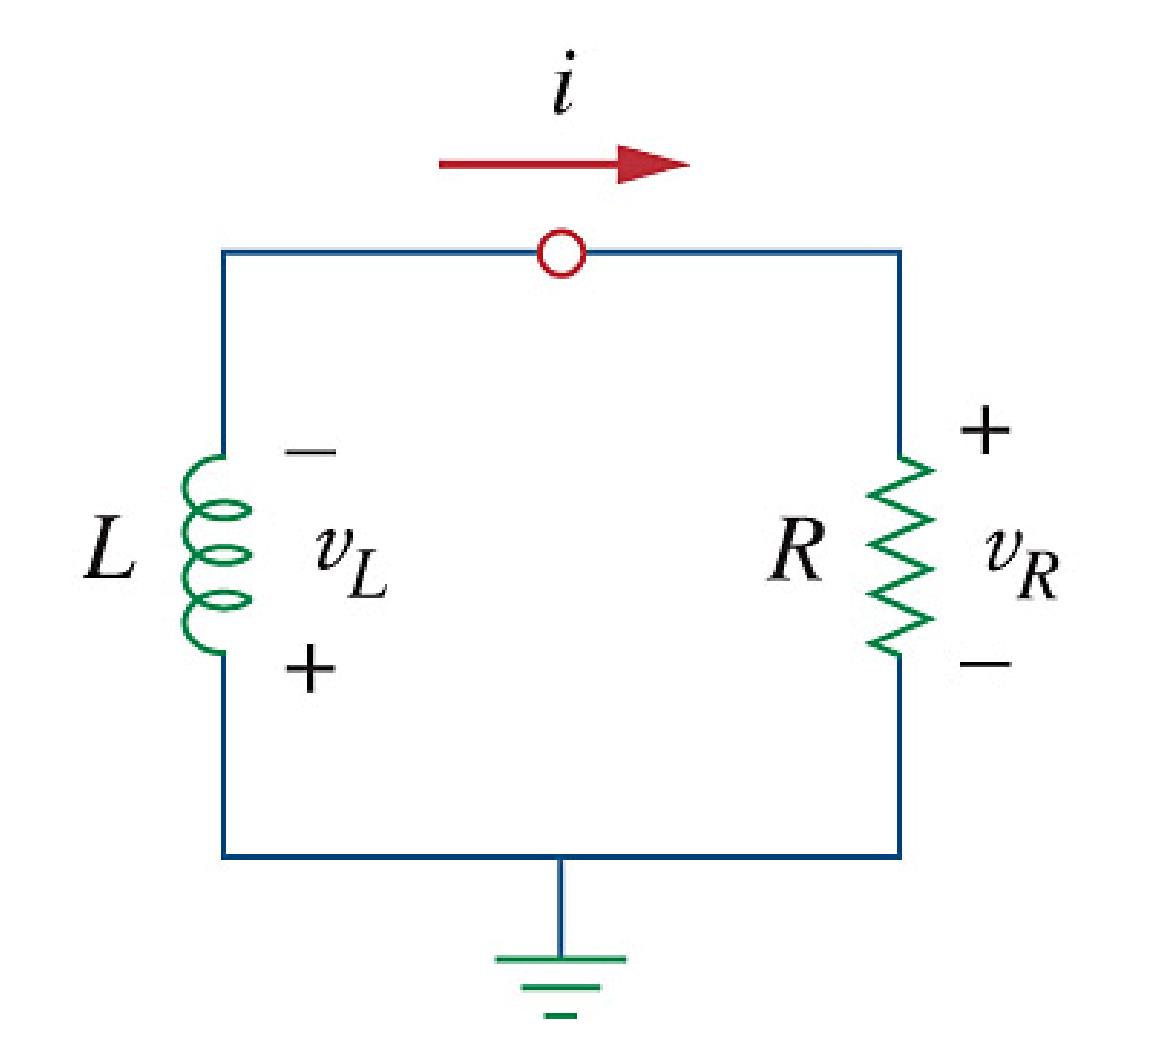
\includegraphics[width=0.35\textwidth]{img_1order/2_source-free_RL.jpg}
        \end{figure}
        \\
        (1) Find initial voltage $v_0$ & (1) Find initial voltage $i_0$\\
        (2) Find time constant $\tau=RC$ & (2) Find time constant $\tau=L/R$\\
        (3) Obtain $v_c$, then $i_c$, $v_R$, $i_R$ & (3) Obtain $i_L$, then $v_L$, $v_R$, $i_R$\\
        % \bottomrule
    \end{tabular}
    % \end{small}
\end{table}

\end{frame}

%%%%%%%%%%%%%%%%%%%%%%%%%%%%%
% \subsection{Circuits wit Step Input}
\begin{frame}{Circuits with Step Input (I) Response}

\begin{table}[]
    \centering
    \setlength{\tabcolsep}{5mm}
    \begin{small}
    
    \begin{tabular}{c|c}
        % \toprule
        \textbf{Step-input RC} & \textbf{Step-input RL}\\
        \begin{figure}
        \centering
        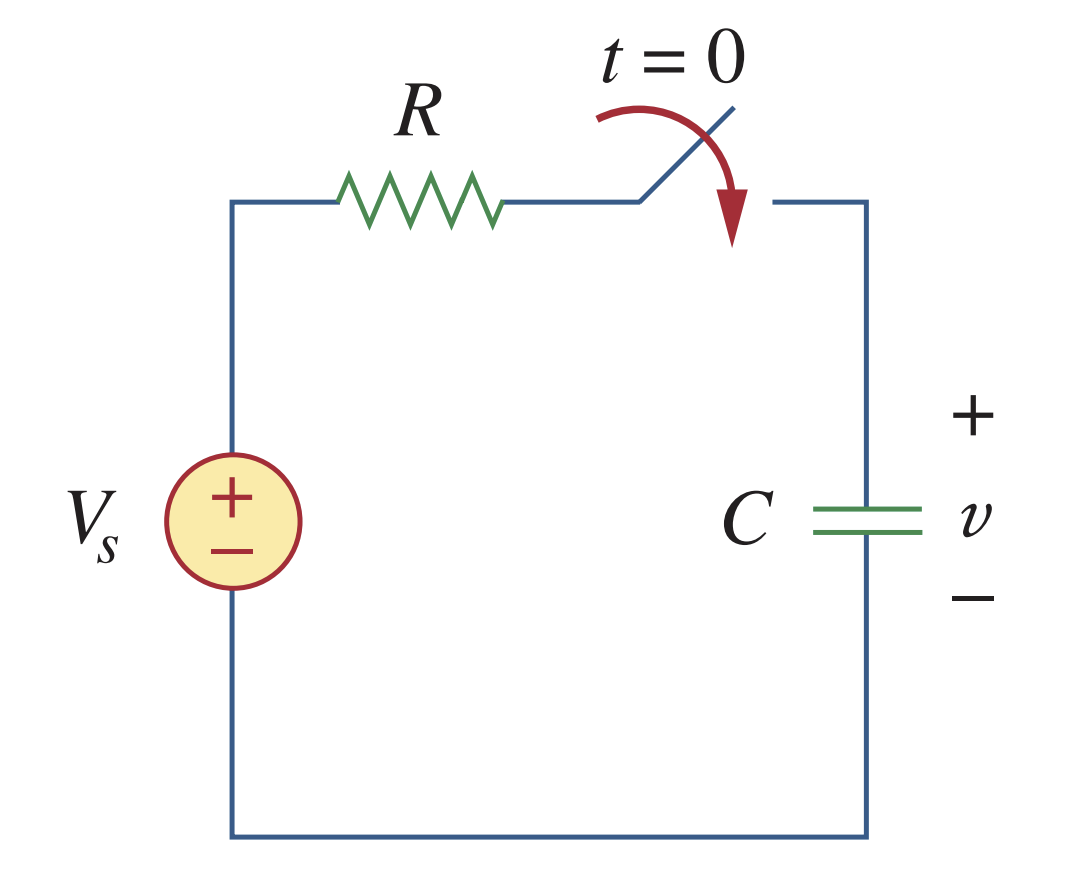
\includegraphics[width=0.35\textwidth]{img_1order/7_stepinputRC.png}
        \end{figure}
        &
        \begin{figure}
        \centering
        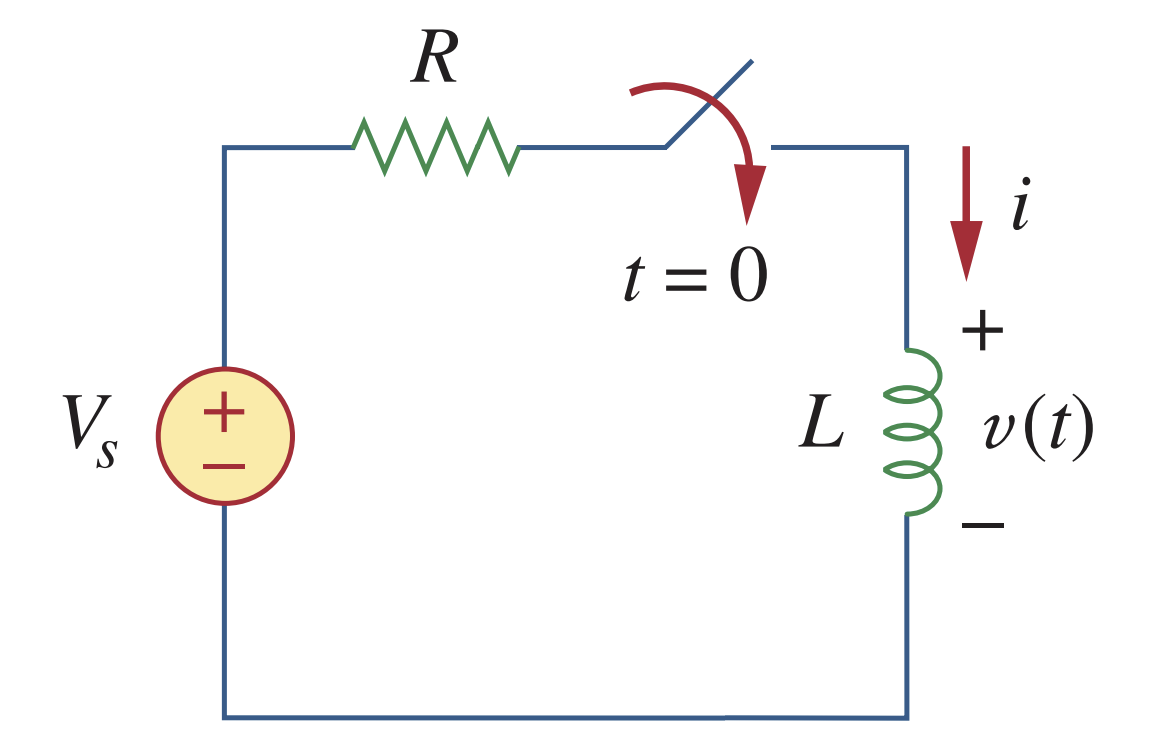
\includegraphics[width=0.34\textwidth]{img_1order/8_stepinputRL.png}
        \end{figure}
        \\
        Initial condition:&Initial condition:\\
        $v(0^+)=v(0^-)=V_0$&$i(0^+)=i(0^-)=I_0$\\
        &\\
        Equation:&Equation:\\
        (KVL) $(C\frac{dv}{dt}R+v=V_s)$&(KCL) $iR+L\frac{di}{dt}=V_s$\\
        &\\
        Response:&Response:\\
        $v(t)=V_s + (V_0-V_s)e^{-t/\tau}$&$i(t)=\frac{V_s}{R} + (I_0-\frac{V_s}{R})e^{-t/\tau}$\\
        
        % \bottomrule
    \end{tabular}
            
    \end{small}
\end{table}

\end{frame}

%%%%%%%%%%%%%%%%%%%%%%%%%%%%%
\begin{frame}{Circuits with Step Input (II) Interpretation of Response}

There are three ways to look at the result.

Take $v(t)=V_s + (V_0-V_s)e^{-t/\tau}$ as example,

\begin{table}[]
    \centering
    \begin{small}
    \begin{tabular}{ccc}
        \toprule
        Interpretation & First component & Second component\\
        \midrule
        $v(t)=v_n(t)+v_f(t)$&$v_n(t)=(V_o-V_s)e^{-t/\tau}$&$v_f(t)=V_s$\\
        &Natural response&Forced response\\
        $v(t)=v_t(t)+v_{ss}(t)$&$v_t(t)=(V_o-V_s)e^{-t/\tau}$&$v_{ss}(t)=V_s$\\
        &Temporary response& Steady-state response\\
        $v(t)=v_{zp}(t)+v_{zs}(t)$&$v_{zp}(t)=V_0e^{t/\tau}$&$v_{zs}(t)=(1-e^{-t/\tau})V_s$\\
        &Zero-input response&Zero-state response\\
        \bottomrule
    \end{tabular}
    \end{small}
    
\end{table}


\end{frame}

%%%%%%%%%%%%%%%%%%%%%%%%%%%%%
\begin{frame}{Circuits with Step Input (III) General Steps}

\begin{table}[]
    \centering
    \setlength{\tabcolsep}{4mm}
    % \begin{small}
    \begin{tabular}{c|c}
        % \toprule
        \textbf{Step-input RC} & \textbf{Step-input RL}\\
        % \midrule
        \begin{figure}
        \centering
        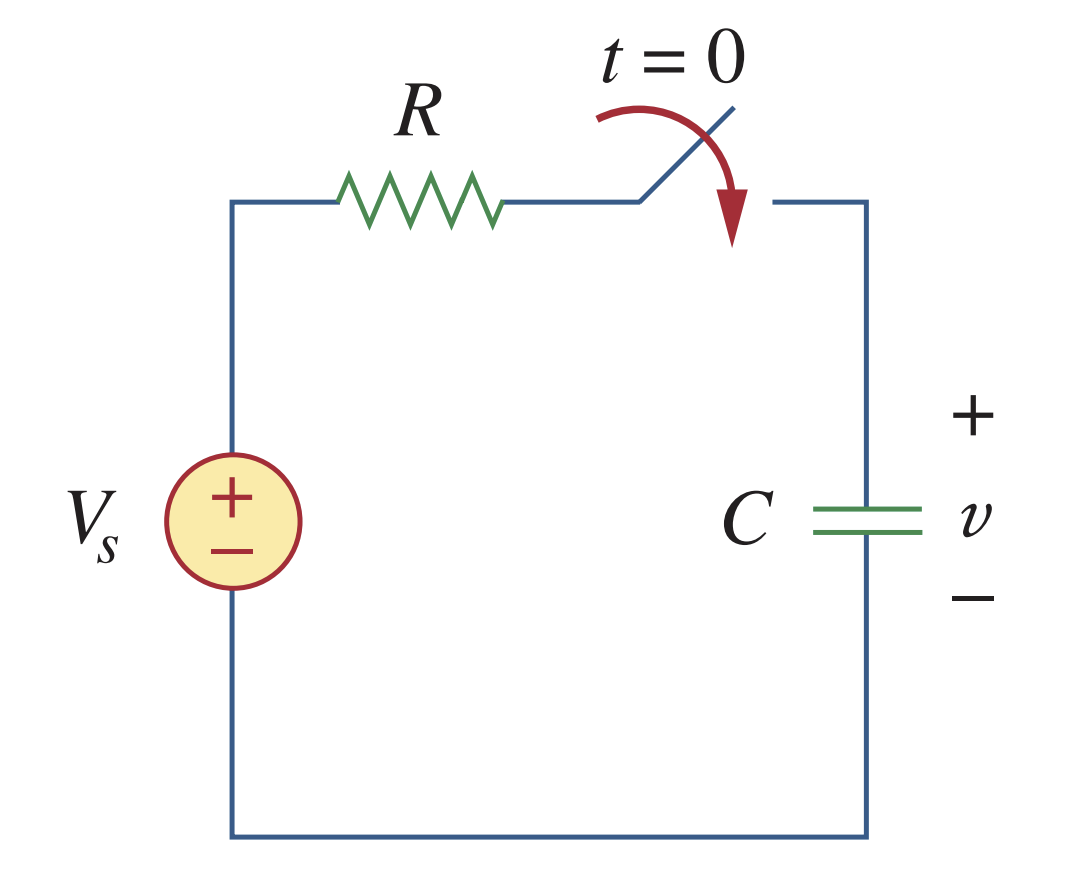
\includegraphics[width=0.35\textwidth]{img_1order/7_stepinputRC.png}
        \end{figure}
        &
        \begin{figure}
        \centering
        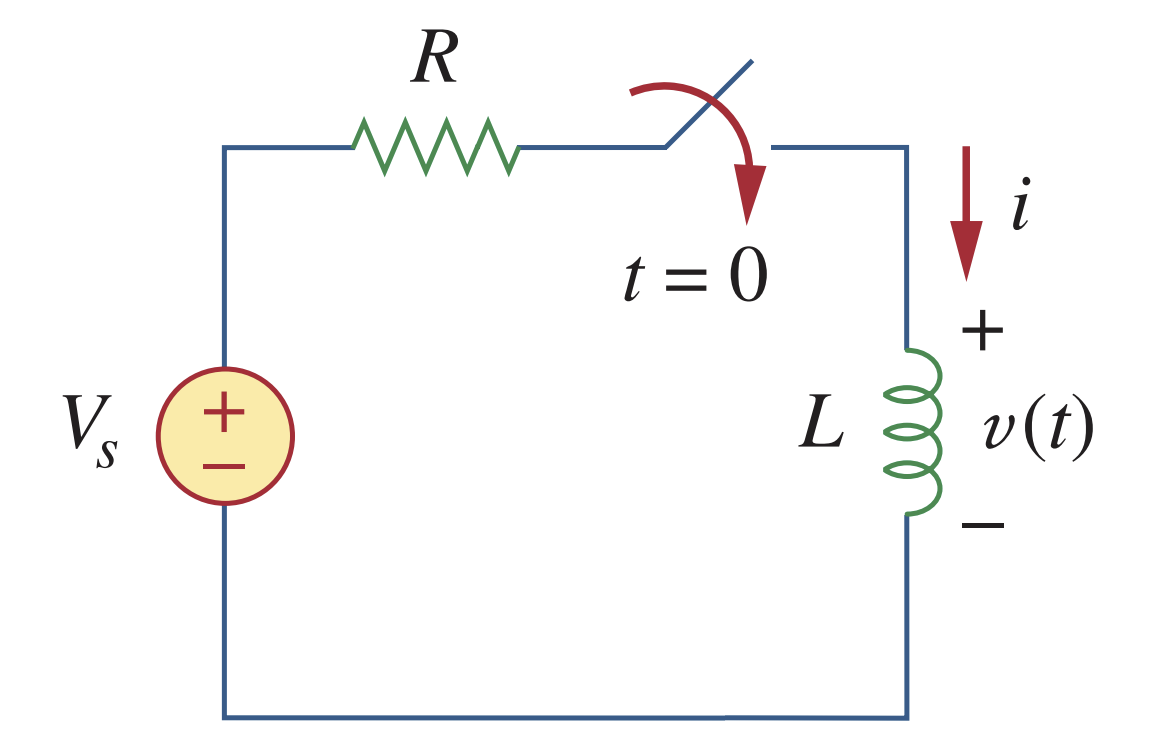
\includegraphics[width=0.34\textwidth]{img_1order/8_stepinputRL.png}
        \end{figure}
        \\

        (1) Find initial voltage $v(0^+)$ & (1) Find initial current $i(0^+)$\\
        (2) Find final voltage $v(\infty)$ & (2) Find find current $i(\infty)$\\
        (3) Find time constant & (3) Find time constant\\
        % \bottomrule
    \end{tabular}
    % \end{small}
    
\end{table}


\end{frame}


%%%%%%%%%%%%%%%%%%%%%%%%%%%%%

\begin{frame}{General Formula for First-Order Circuits}


\color{red}
General formula for RC:
$$v(t) = v(\infty)+\left[v(0^+)-v(\infty)\right]e^{-t/\tau}$$
General formula for RL:
$$i(t) = i(\infty)+\left[i(0^+)-i(\infty)\right]e^{-t/\tau}$$
\color{black}

\end{frame}

%%%%%%%%%%%%%%%%%%%%%%%%%%%%%

\begin{frame}{Exercise}

%TODO: 改一下格式
Find $i_0,\ v_o$ and $i$ for all time, assuming that the switch was open for a long time.
\begin{figure}
\centering
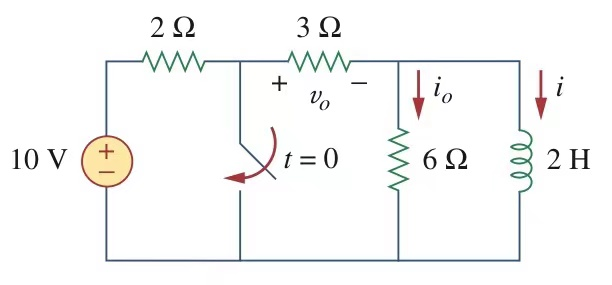
\includegraphics[width=3in]{img_1order/ex3.jpg}
\end{figure}
\end{frame}

%%%%%%%%%%%%%%%%%%%%%%%%%%%%%

% \begin{frame}{Exercise}



% \end{frame}

%%%%%%%%%%%%%%%%%%%%%%%%%%%%%%%%%%%%%%%%%%%%%%%%%%%
% 2ND-ORDER CIRCUITS
\section{Second-Order Circuit}
% \subsection{Find Initial and FInal Values}

%%%%%%%%%%%%%%%%%%%%%%%%%%%%%

\begin{frame}{Introduction}

Definition: a second-order circuit is a circuit that consists of resistors and \textbf{TWO} capacitors/inductors after circuit simplification.

\

Workflow to solve 2nd-order circuits:
\begin{center}
    Find initial and final values and its derivative
    
    $\downarrow$

    List differential equation and find its solution

    $\downarrow$

    Use initial and final values to determine the coefficients in the solution
    
\end{center}

\end{frame}

%%%%%%%%%%%%%%%%%%%%%%%%%%%%%
\begin{frame}{Initial and Final Values}
    \begin{itemize}
        \item $v(0)$,$i(0)$,$v(\infty)$,$i(\infty)$: same method as the first-order circuit.
        \item $dv(0)/dt=I_C/C$ (Trick here is to use the property that the current across an inductor cannot change abruptly.)
        \item $di(0)/dt=V_L/L$ (Trick here is to use the property that the voltage of a capacitor cannot change abruptly.)
    \end{itemize}
    \begin{alertblock}{Caution}
    Please do care about the polarity when calculating the initial derivatives! You should always remember that current flows from high voltage to low voltage.  
    
    \end{alertblock}

    
\end{frame}

%%%%%%%%%%%%%%%%%%%%%%%%%%%%%

\begin{frame}{Basic RLC Circuits}

\begin{table}[]
    \centering
    \begin{tabular}{c|cc}
    \toprule
         &Series connection& Parallel connection  \\
    % \midrule
    \hline
    &&\\
    &(By KVL)&(By KCL)\\
         Source-free& $\frac{d^2i}{dt^2}+\frac{R}{L}\frac{di}{dt}+\frac{1}{LC}i=0$ & $\frac{d^2v}{dt^2}+\frac{1}{RC}\frac{dv}{dt}+\frac{1}{LC}v=0$\\
         &
        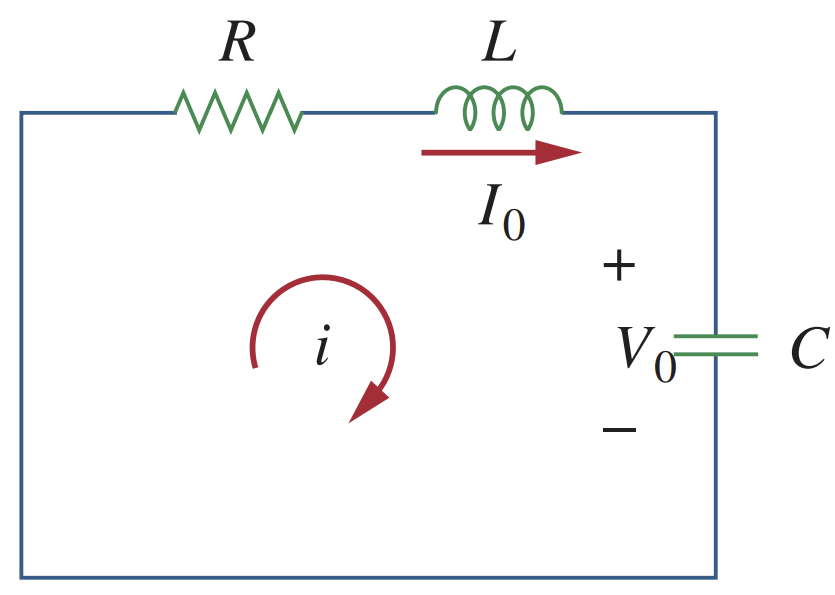
\includegraphics[width=0.27\textwidth]{img_2order/4_sourcefreeseries.png}
         &
         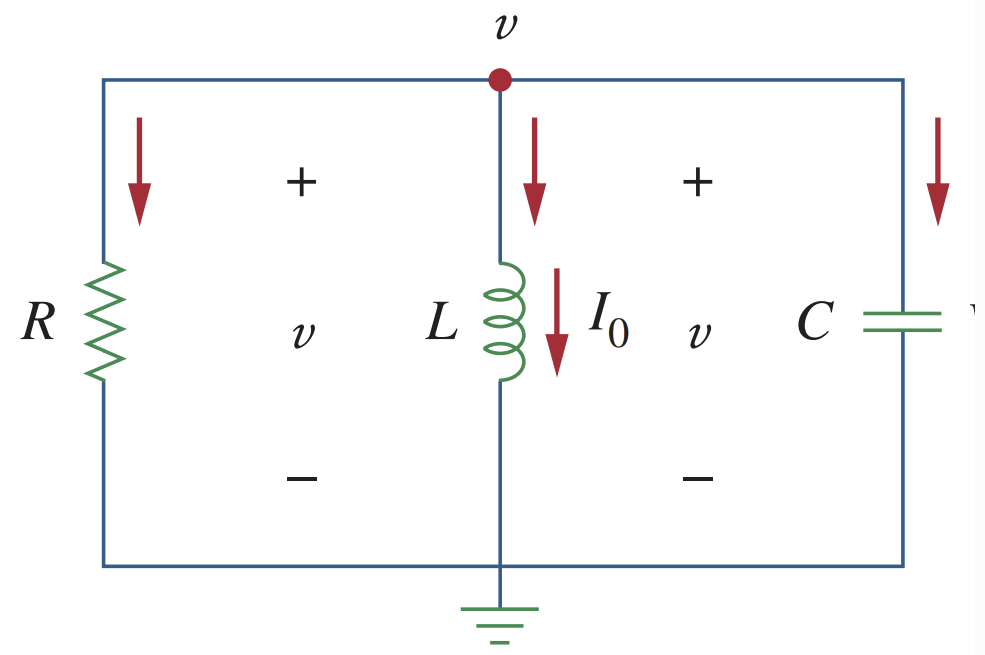
\includegraphics[width=0.3\textwidth]{img_2order/5_sourcefreeparallel.png}
         \\
          &(By KVL)&(By KCL)\\
        Step input& $\frac{d^2v}{dt^2}+\frac{R}{L}\frac{dv}{dt}+\frac{1}{LC}v=V_s$ & $\frac{d^2i}{dt^2}+\frac{1}{RC}\frac{di}{dt}+\frac{1}{LC}i=I_s$\\
          &
         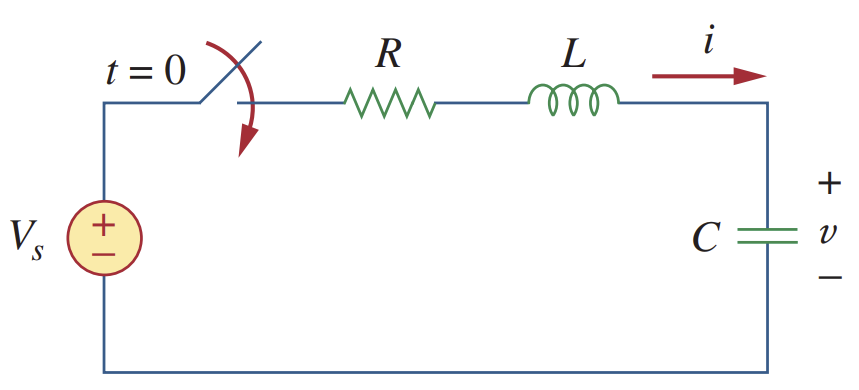
\includegraphics[width=0.35\textwidth]{img_2order/6_stepresponseseries.png}
         &
         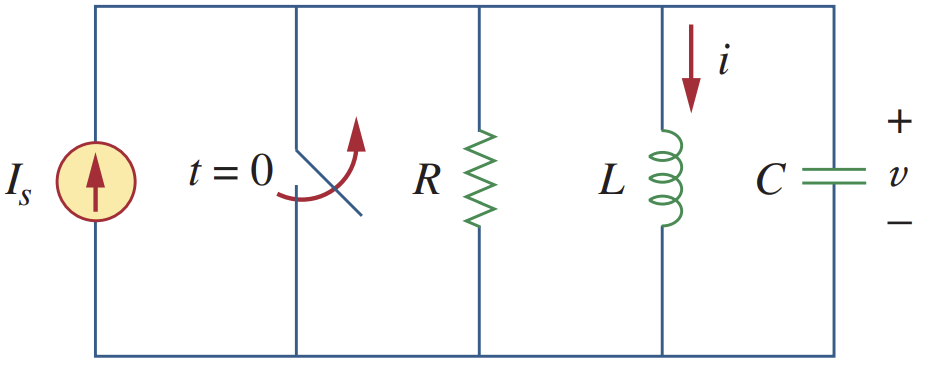
\includegraphics[width=0.32\textwidth]{img_2order/7_stepresponseparallel.png}
         \\
         \bottomrule
    \end{tabular}
\end{table}
    
\end{frame}

%%%%%%%%%%%%%%%%%%%%%%%%%%%%%

\begin{frame}{Solving 2nd-Order Differential Equations}

Through analysis we will obtain the differential equation for $x$, 
\begin{itemize}
    \item For source-free circuits, $a\frac{d^2x}{dt^2}+b\frac{dx}{dt}+cx=0$

    (homogeneous, 2nd-order, const coefficient)
    \item For step input circuits, $a\frac{d^2x}{dt^2}+b\frac{dx}{dt}+cx=X_0$

    (non-homogeneous, 2nd-order, const coefficient)
\end{itemize}

\begin{table}[]
    \centering
    \begin{small}
           
    \begin{tabular}{ccc}
        \toprule
        Underdamped & Critically damped & Overdamped\\
        \midrule
        $b^2-4ac < 0$& $b^2-4ac=0$ & $b^2-4ac>0$ \\ 
        No root & One root $s$ & Two roots $s_1$, $s_2$ \\
        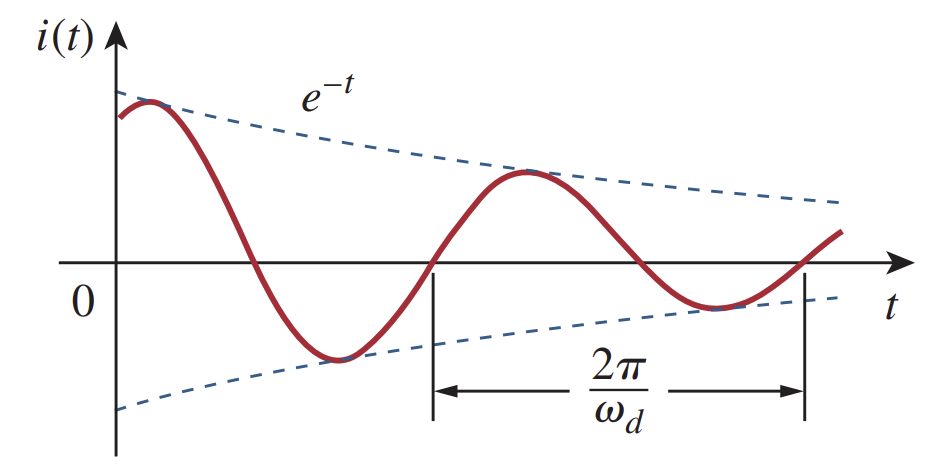
\includegraphics[width=0.3\textwidth]{img_2order/3_underdamped.png}
        &
        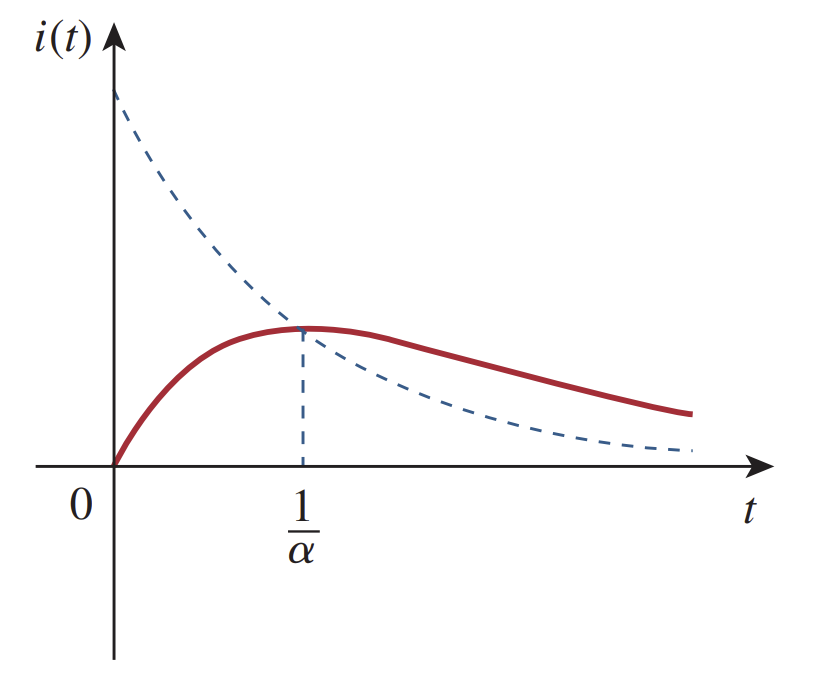
\includegraphics[width=0.25\textwidth]{img_2order/2_criticallydamped.png}
        &
        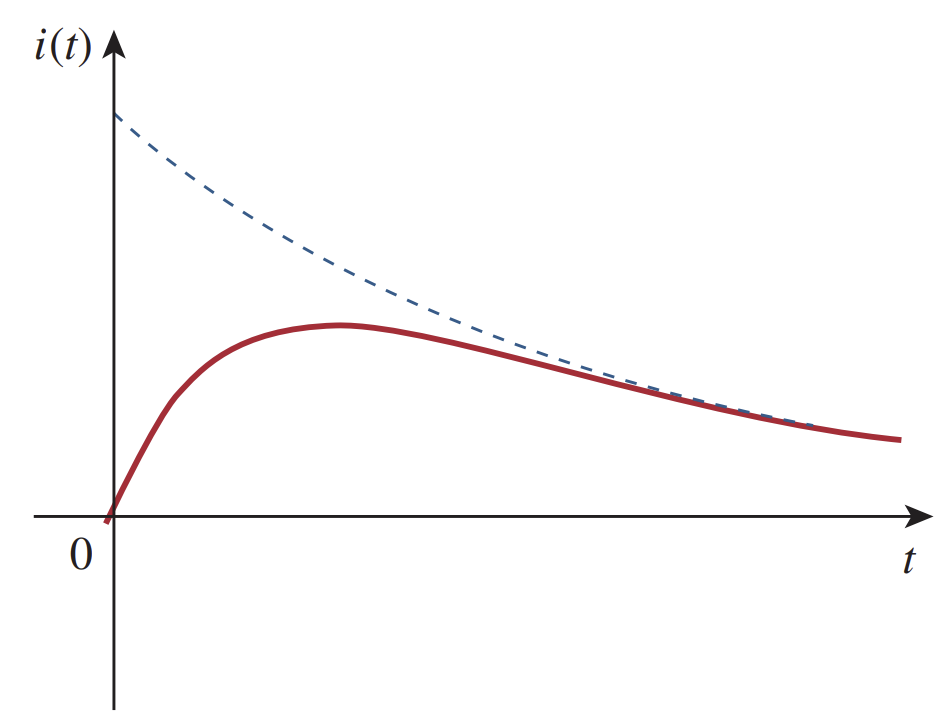
\includegraphics[width=0.25\textwidth]{img_2order/1_overdamped.png}
        \\
         \bottomrule
    \end{tabular}
    \end{small}
\end{table}

    
\end{frame}


%%%%%%%%%%%%%%%%%%%%%%%%%%%%%

\begin{frame}{Solving 2nd-Order Differential Equations}
For $a\frac{d^2x}{dt^2}+b\frac{dx}{dt}+cx=0$ (homogeneous),
\begin{itemize}
    \item No root:
    $$r=-\frac{b}{2a}, \omega = \frac{\sqrt{4ac-b^2}}{2a}$$
    $$x(t)=e^{rt}(C_1\sin \omega t + C_2 \cos \omega t) $$
    \item One root $s$:
    $$x(t)=(C_1+C_2t)e^{st}$$
    \item To roots $s_1$, $s_2$:
    $$x(t)=C_1e^{s_1t}+C_2e^{s_2t}$$
\end{itemize}
For $a\frac{d^2x}{dt^2}+b\frac{dx}{dt}+cx=X_0$ (non-homogeneous), adopt
$$x(t)=x_{homogeneous}(t) + x_{particular}(t)$$
\end{frame}

%%%%%%%%%%%%%%%%%%%%%%%%%%%%%

\begin{frame}{General Steps for Second-Order Circuits}
What we want: $v(t)$ or $i(t)$ of some part of the circuit
\begin{itemize}
    \item For source-free circuit:
    \begin{enumerate}
        \item Draw the circuit for $t < 0$, obtain $i(0^+)$ and $v(0^+)$
        \item Draw the circuit for $t>0$, list equations to obtain $\frac{di(0^+)}{dt}$ or $\frac{dv(0^+)}{dt}$
        \item Get the differential equation for the variable we want to study 
        
        $\longrightarrow$ Judge how many roots in its characteristic equation

        $\longrightarrow$ Select the form of solution (with two coefficients unsolved)

        \item Use the initial conditions to solve the two coefficients $C_1$, $C_2$
    \end{enumerate}

    \item For step-input circuit:
    \begin{enumerate}
        \item Follow the same steps to obtain the differential equation
        \item \textbf{Solve its corresponding homogeneous differential equation $y_{homogeneous}$} (with two coefficients unsolved)
        \item Find a \textbf{constant} particular solution, i.e. $y_{particular} = C$ such that $a\times 0 + b\times 0 + c \times C = X_0 \Rightarrow C = X_0/c$
        \item General solution $x = x_{homogeneous} + x_{particular}$
        \item Use the initial conditions to solve the two coefficients $C_1$, $C_2$ 
    \end{enumerate}
    
\end{itemize}
    
\end{frame}

%%%%%%%%%%%%%%%%%%%%%%%%%%%%%

\begin{frame}{General Steps for Second-Order Circuits}

Tips for finding the differential equation:
\begin{itemize}
    \item Start from KCL or KVL?

    Better to try KVL in a scenario similar to series connection, and to try KCL in a scenario similar to parallel connection
    
    \item Take advantage of the property of capacitor \& inductor:
    \begin{itemize}
        \item There might be both $v$ and $i$ in the original equation, but only one of them is desired.
    
        \item So consider using $i=C\frac{dv}{dt}$ and $v=L\frac{di}{dt}$ to ``kill" one of them
    \end{itemize}
    
\end{itemize}

    
\end{frame}

%%%%%%%%%%%%%%%%%%%%%%%%%%%%%

\begin{frame}{Exercise}
The switch in the circuit has been in position for a long time. At $t=0$ the switch move instantaneously to position b. Find $i(t)$.
\begin{figure}
\centering
\includegraphics[width=0.6\textwidth]{img_2order/ex.png}
\end{figure}

\end{frame}

% %%%%%%%%%%%%%%%%%%%%%%%%%%%%%
% \begin{frame}{Exercise}
    
% \end{frame}


% %%%%%%%%%%%%%%%%%%%%%%%%%%%%%
% \begin{frame}{Exercise}
    
% \end{frame}

%%%%%%%%%%%%%%%%%%%%%%%%%%%%%%%%%%%%%%%%%%%%%%%%%%%
% DUALITY


\section{Duality}
\begin{frame}{Dual Pairs}
\begin{table}[]
    \centering
    \setlength{\tabcolsep}{7mm}
    \begin{tabular}{ccc}
         Resistance $R$ &$\longleftrightarrow$& Conductance $G$ \\
         Inductance $L$&$\longleftrightarrow$& Capacitance $C$ \\
         Voltage $v$ &$\longleftrightarrow$& Current $i$ \\
         Node &$\longleftrightarrow$& Mesh \\
         Serie path &$\longleftrightarrow$& Parallel path \\
         Open circuit &$\longleftrightarrow$& Short circuit \\
         KVL &$\longleftrightarrow$& KCL \\
         Thevenin &$\longleftrightarrow$& Norton \\
    \end{tabular}
    % \caption{Caption}
    % \label{tab:my_label}
\end{table}
\end{frame}

%%%%%%%%%%%%%%%%%%%%%%%%%%%%%

\begin{frame}{Steps to Draw Dual Circuits}

    \begin{itemize}
        \item Place a node at the center of each mesh of the given circuit. Place the reference node (the ground) of the dual circuit outside the given circuit.
        \item Draw lines between the nodes such that each line crosses an element. Replace that element by its dual.
        \item To determine the polarity of voltage sources and direction of current sources, follow this rule: A voltage source that produces a positive (clockwise) mesh current has as its dual a current source whose reference direction is from the ground to the non-reference node.
    \end{itemize}
\end{frame}




%%%%%%%%%%%%%%%%%%%%%%%%%%%%%%%%%%%%%%%%%%%%%%%%%%%
\begin{frame}
\frametitle{References}
\begin{enumerate}
\item 2023 Summer VE215 slides, Rui Yang
\item Fundamentals of Electric Circuits, 5th e, Sadiku, Matthew
\item 2022 Fall RC4, Zhiyu Zhou
\item 2022 Fall Mid RC, Zhiyu Zhou, Yifei Cai, Yuxuan Peng
\end{enumerate}
\end{frame}


\begin{frame}
\Huge{\centerline{Thank you!}}
\end{frame}


\end{document}
